% Options for packages loaded elsewhere
% Options for packages loaded elsewhere
\PassOptionsToPackage{unicode}{hyperref}
\PassOptionsToPackage{hyphens}{url}
%
\documentclass[
  english,
  russian,
  12pt,
  a4paper,
  DIV=11,
  numbers=noendperiod]{scrreprt}
\usepackage{xcolor}
\usepackage{amsmath,amssymb}
\setcounter{secnumdepth}{5}
\usepackage{iftex}
\ifPDFTeX
  \usepackage[T1]{fontenc}
  \usepackage[utf8]{inputenc}
  \usepackage{textcomp} % provide euro and other symbols
\else % if luatex or xetex
  \usepackage{unicode-math} % this also loads fontspec
  \defaultfontfeatures{Scale=MatchLowercase}
  \defaultfontfeatures[\rmfamily]{Ligatures=TeX,Scale=1}
\fi
\usepackage{lmodern}
\ifPDFTeX\else
  % xetex/luatex font selection
\fi
% Use upquote if available, for straight quotes in verbatim environments
\IfFileExists{upquote.sty}{\usepackage{upquote}}{}
\IfFileExists{microtype.sty}{% use microtype if available
  \usepackage[]{microtype}
  \UseMicrotypeSet[protrusion]{basicmath} % disable protrusion for tt fonts
}{}
\usepackage{setspace}
% Make \paragraph and \subparagraph free-standing
\makeatletter
\ifx\paragraph\undefined\else
  \let\oldparagraph\paragraph
  \renewcommand{\paragraph}{
    \@ifstar
      \xxxParagraphStar
      \xxxParagraphNoStar
  }
  \newcommand{\xxxParagraphStar}[1]{\oldparagraph*{#1}\mbox{}}
  \newcommand{\xxxParagraphNoStar}[1]{\oldparagraph{#1}\mbox{}}
\fi
\ifx\subparagraph\undefined\else
  \let\oldsubparagraph\subparagraph
  \renewcommand{\subparagraph}{
    \@ifstar
      \xxxSubParagraphStar
      \xxxSubParagraphNoStar
  }
  \newcommand{\xxxSubParagraphStar}[1]{\oldsubparagraph*{#1}\mbox{}}
  \newcommand{\xxxSubParagraphNoStar}[1]{\oldsubparagraph{#1}\mbox{}}
\fi
\makeatother


\usepackage{longtable,booktabs,array}
\usepackage{calc} % for calculating minipage widths
% Correct order of tables after \paragraph or \subparagraph
\usepackage{etoolbox}
\makeatletter
\patchcmd\longtable{\par}{\if@noskipsec\mbox{}\fi\par}{}{}
\makeatother
% Allow footnotes in longtable head/foot
\IfFileExists{footnotehyper.sty}{\usepackage{footnotehyper}}{\usepackage{footnote}}
\makesavenoteenv{longtable}
\usepackage{graphicx}
\makeatletter
\newsavebox\pandoc@box
\newcommand*\pandocbounded[1]{% scales image to fit in text height/width
  \sbox\pandoc@box{#1}%
  \Gscale@div\@tempa{\textheight}{\dimexpr\ht\pandoc@box+\dp\pandoc@box\relax}%
  \Gscale@div\@tempb{\linewidth}{\wd\pandoc@box}%
  \ifdim\@tempb\p@<\@tempa\p@\let\@tempa\@tempb\fi% select the smaller of both
  \ifdim\@tempa\p@<\p@\scalebox{\@tempa}{\usebox\pandoc@box}%
  \else\usebox{\pandoc@box}%
  \fi%
}
% Set default figure placement to htbp
\def\fps@figure{htbp}
\makeatother



\ifLuaTeX
\usepackage[bidi=basic,provide=*]{babel}
\else
\usepackage[bidi=default,provide=*]{babel}
\fi
% get rid of language-specific shorthands (see #6817):
\let\LanguageShortHands\languageshorthands
\def\languageshorthands#1{}


\setlength{\emergencystretch}{3em} % prevent overfull lines

\providecommand{\tightlist}{%
  \setlength{\itemsep}{0pt}\setlength{\parskip}{0pt}}



 
\usepackage[backend=biber,langhook=extras,autolang=other*]{biblatex}
\addbibresource{bib/cite.bib}

\usepackage[]{csquotes}

\KOMAoption{captions}{tableheading}
\usepackage{indentfirst}
\usepackage{float}
\floatplacement{figure}{H}
\usepackage{libertine}
\makeatletter
\@ifpackageloaded{caption}{}{\usepackage{caption}}
\AtBeginDocument{%
\ifdefined\contentsname
  \renewcommand*\contentsname{Содержание}
\else
  \newcommand\contentsname{Содержание}
\fi
\ifdefined\listfigurename
  \renewcommand*\listfigurename{Список иллюстраций}
\else
  \newcommand\listfigurename{Список иллюстраций}
\fi
\ifdefined\listtablename
  \renewcommand*\listtablename{Список таблиц}
\else
  \newcommand\listtablename{Список таблиц}
\fi
\ifdefined\figurename
  \renewcommand*\figurename{Рисунок}
\else
  \newcommand\figurename{Рисунок}
\fi
\ifdefined\tablename
  \renewcommand*\tablename{Таблица}
\else
  \newcommand\tablename{Таблица}
\fi
}
\@ifpackageloaded{float}{}{\usepackage{float}}
\floatstyle{ruled}
\@ifundefined{c@chapter}{\newfloat{codelisting}{h}{lop}}{\newfloat{codelisting}{h}{lop}[chapter]}
\floatname{codelisting}{Список}
\newcommand*\listoflistings{\listof{codelisting}{Листинги}}
\makeatother
\makeatletter
\makeatother
\makeatletter
\@ifpackageloaded{caption}{}{\usepackage{caption}}
\@ifpackageloaded{subcaption}{}{\usepackage{subcaption}}
\makeatother
\usepackage{bookmark}
\IfFileExists{xurl.sty}{\usepackage{xurl}}{} % add URL line breaks if available
\urlstyle{same}
\hypersetup{
  pdftitle={Отчёт по лабораторной работе 4},
  pdfauthor={Калашникова Ольга Сергеевна},
  pdflang={ru-RU},
  hidelinks,
  pdfcreator={LaTeX via pandoc}}


\title{Отчёт по лабораторной работе 4}
\author{Калашникова Ольга Сергеевна}
\date{}
\begin{document}
\maketitle

\renewcommand*\contentsname{Содержание}
{
\setcounter{tocdepth}{1}
\tableofcontents
}
\listoffigures
\listoftables

\setstretch{1.5}
\chapter{Цель
работы}\label{ux446ux435ux43bux44c-ux440ux430ux431ux43eux442ux44b}

Установка и настройка GNS3 и сопутствующего программного обеспечения.

\chapter{Задание}\label{ux437ux430ux434ux430ux43dux438ux435}

\begin{enumerate}
\def\labelenumi{\arabic{enumi}.}
\item
  Установить GNS3-all-in-one, GNS3 VM, проверить корректность запуска
\item
  Импортировать в GNS3 образ маршрутизатора FRR
\item
  Импортировать в GNS3 образ маршрутизатора VyOS
\end{enumerate}

\chapter{Выполнение лабораторной
работы}\label{ux432ux44bux43fux43eux43bux43dux435ux43dux438ux435-ux43bux430ux431ux43eux440ux430ux442ux43eux440ux43dux43eux439-ux440ux430ux431ux43eux442ux44b}

\section{Установка
GNS3-all-in-one}\label{ux443ux441ux442ux430ux43dux43eux432ux43aux430-gns3-all-in-one}

Скачиваем GNS3 через менеджер пакетов с помощью команды choco install
gns3 -y (рис.~\ref{fig-001}).

\begin{figure}

\centering{

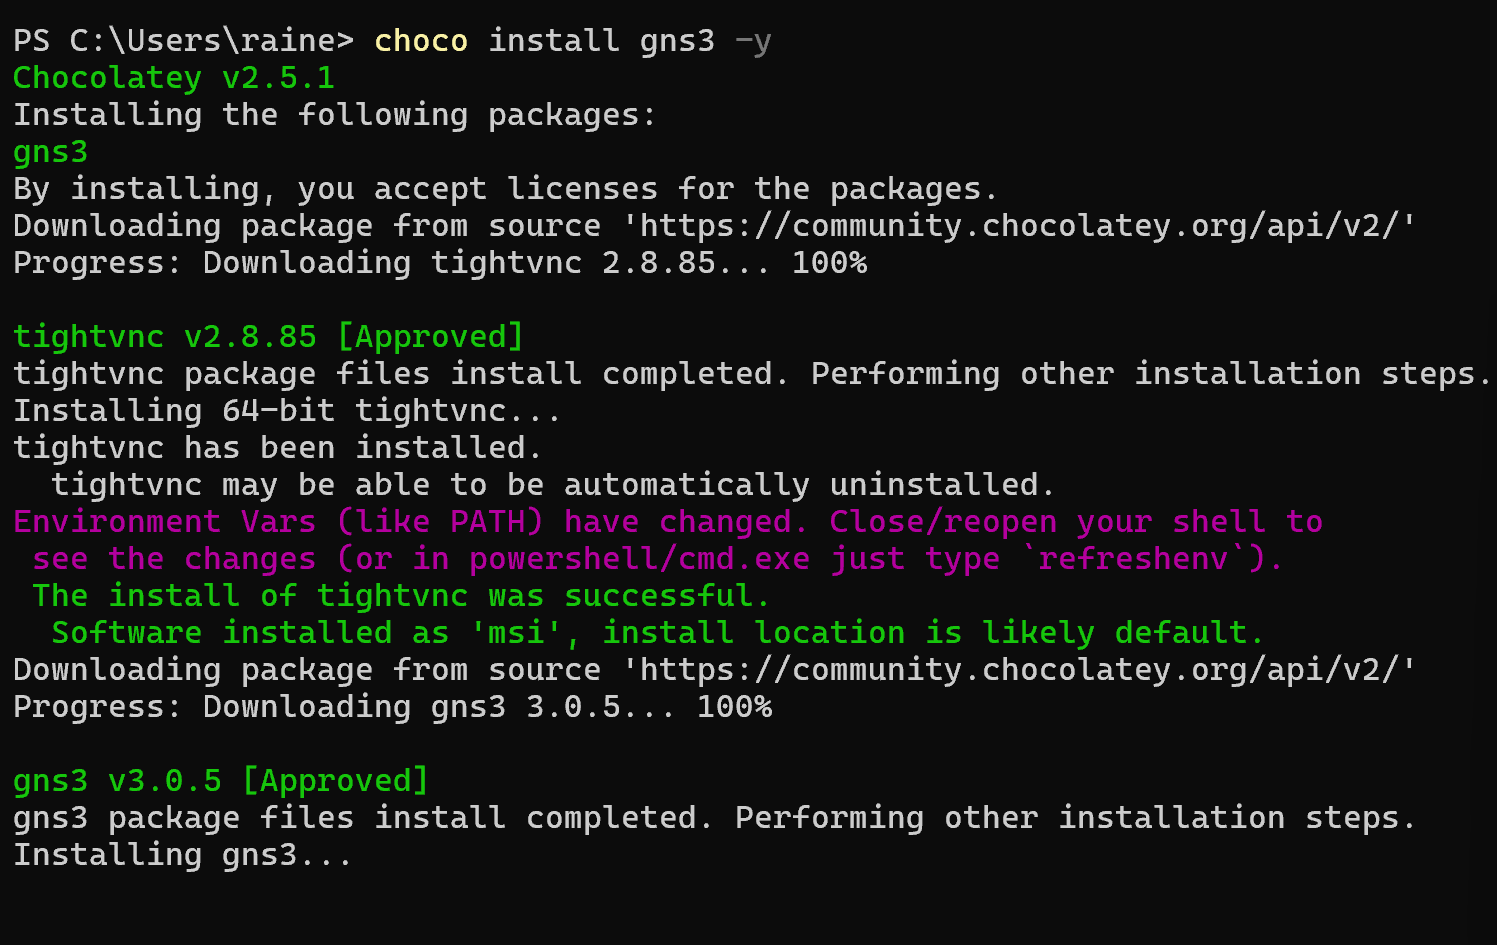
\includegraphics[width=0.7\linewidth,height=\textheight,keepaspectratio]{image/1.png}

}

\caption{\label{fig-001}Установка GNS3}

\end{figure}%

Запускается графическое окно по установке (рис.~\ref{fig-002}).

\begin{figure}

\centering{

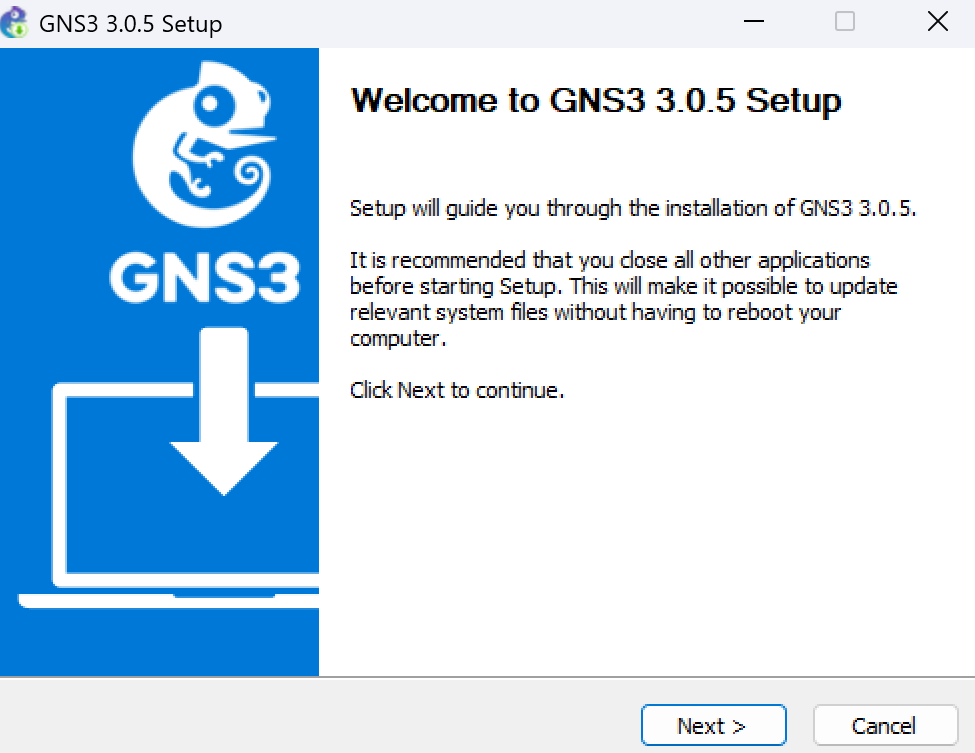
\includegraphics[width=0.7\linewidth,height=\textheight,keepaspectratio]{image/2.png}

}

\caption{\label{fig-002}Графическое окно по установке}

\end{figure}%

В процессе установки при выборе комплектации отмечаем MSVC Runtime,
GNS3-Desktop, GNS3-VM, Tools (рис.~\ref{fig-003}).

\begin{figure}

\centering{

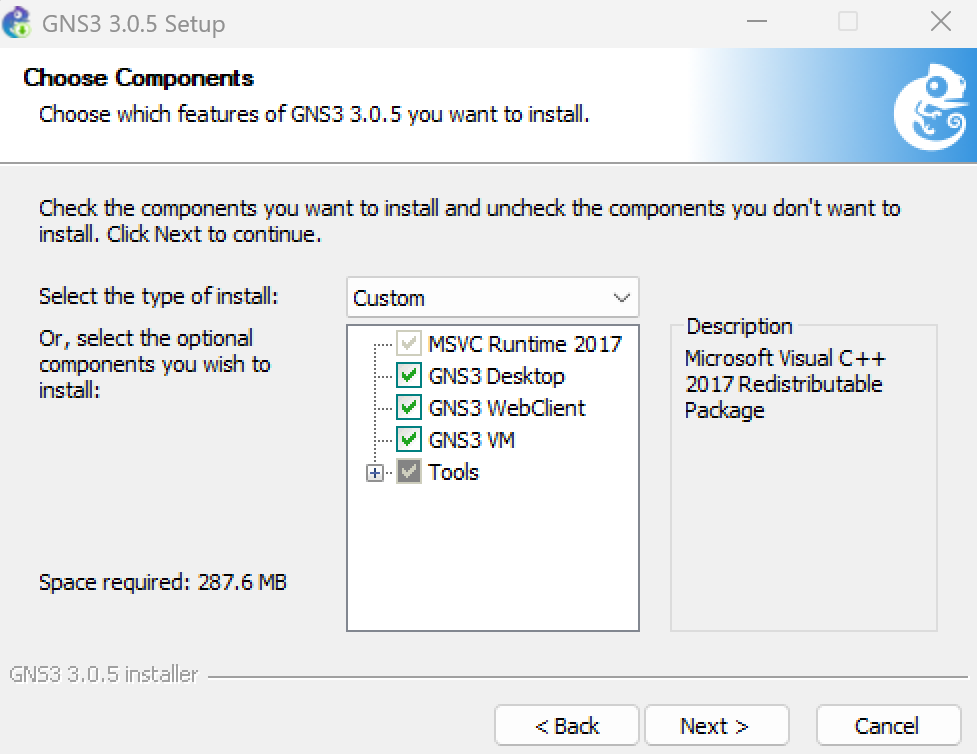
\includegraphics[width=0.7\linewidth,height=\textheight,keepaspectratio]{image/3.png}

}

\caption{\label{fig-003}Выбор комплектации}

\end{figure}%

Дальше требуется отметить тот тип виртуальной машины, через которую в
дальнейшем я буду работать с GNS3. Я указала VirtualBox
(рис.~\ref{fig-004}).

\begin{figure}

\centering{

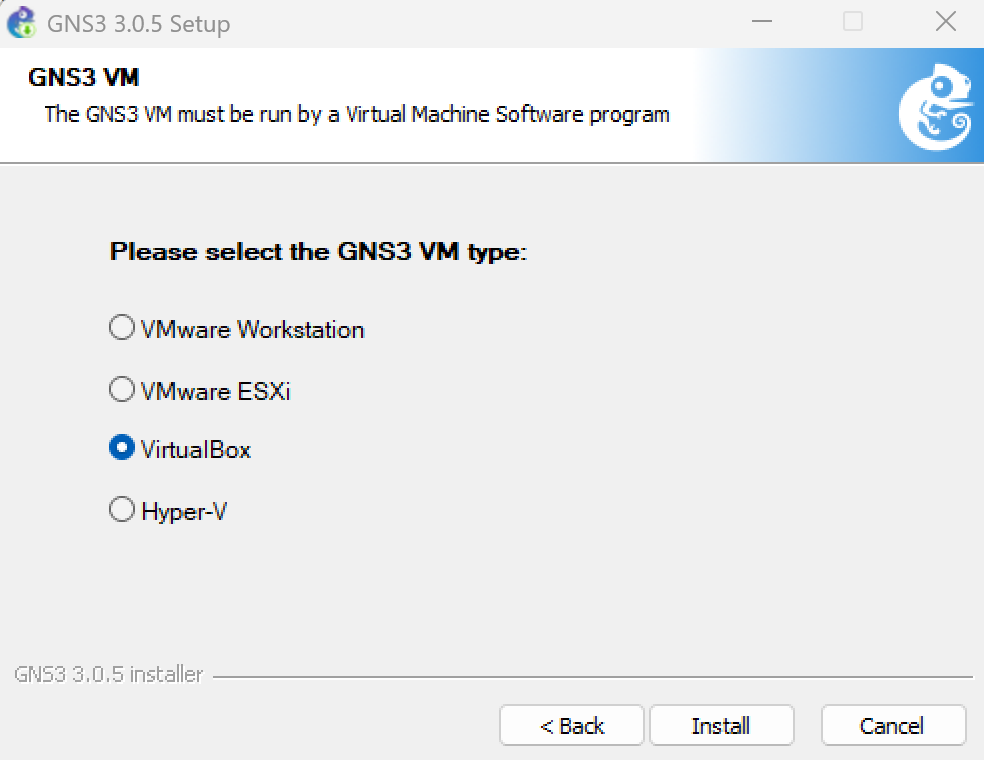
\includegraphics[width=0.7\linewidth,height=\textheight,keepaspectratio]{image/4.png}

}

\caption{\label{fig-004}Выбор типа виртуальной машины}

\end{figure}%

\section{Установка GNS3 VM для
VirtualBox}\label{ux443ux441ux442ux430ux43dux43eux432ux43aux430-gns3-vm-ux434ux43bux44f-virtualbox}

Перейдём в каталог, в который скачан архив с образом виртуальной машины
GNS3.VM.VirtualBox.2.2.54.zip. и распакуем архив с образом
(рис.~\ref{fig-005}).

\begin{figure}

\centering{

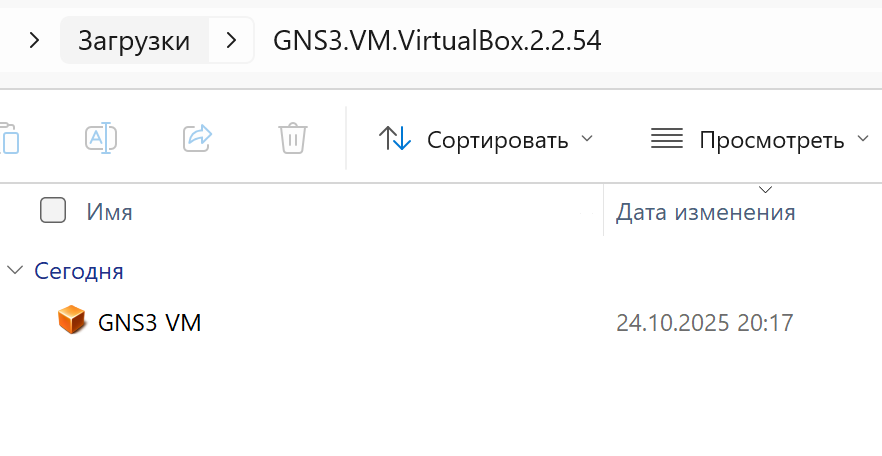
\includegraphics[width=0.7\linewidth,height=\textheight,keepaspectratio]{image/5.png}

}

\caption{\label{fig-005}Распаковка образа}

\end{figure}%

Запустим VirtualBox и выберем Импорт конфигураций. Укажем
месторасположение распакованного образа GNS3 VM.ova
(рис.~\ref{fig-006}).

\begin{figure}

\centering{

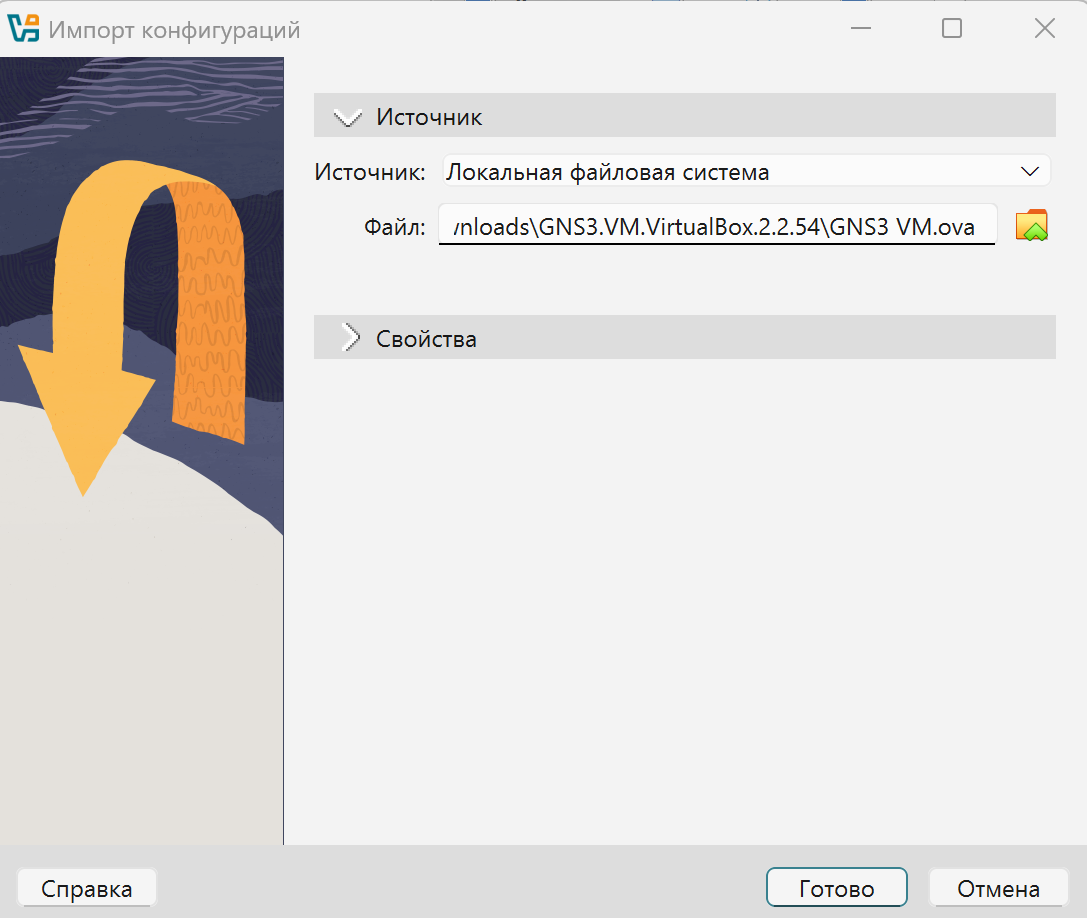
\includegraphics[width=0.7\linewidth,height=\textheight,keepaspectratio]{image/6.png}

}

\caption{\label{fig-006}Импорт конфигураций}

\end{figure}%

В параметрах импорта выберем в политике MAC-адреса «Сгенерировать новые
MAC-адреса всех сетевых адаптеров» (рис.~\ref{fig-007}).

\begin{figure}

\centering{

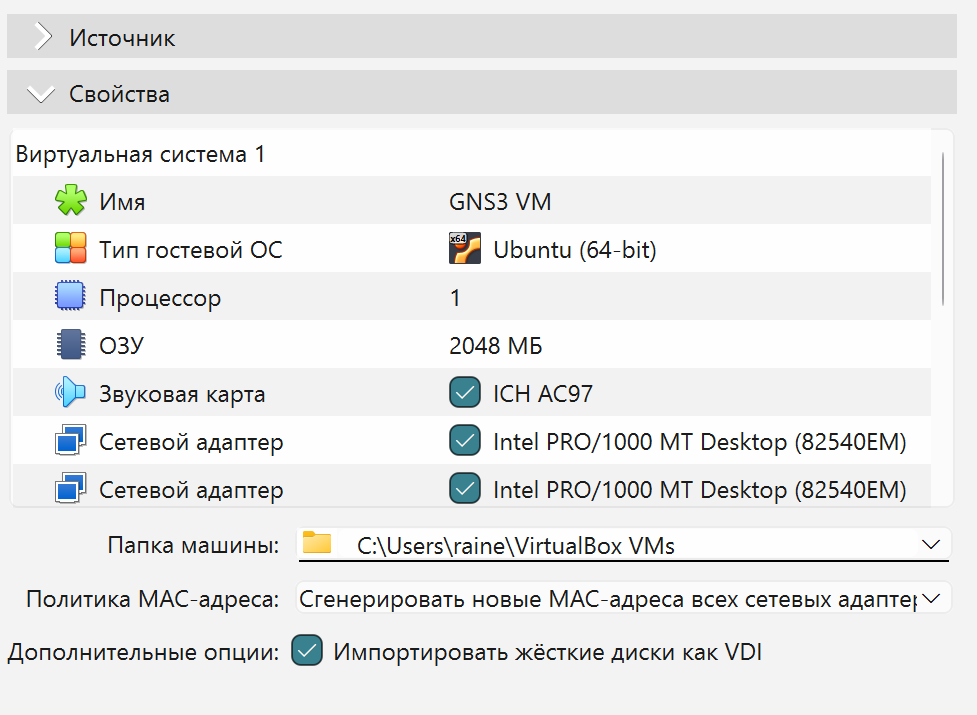
\includegraphics[width=0.7\linewidth,height=\textheight,keepaspectratio]{image/7.png}

}

\caption{\label{fig-007}Редактирование параметров импорта}

\end{figure}%

После импорта виртуальной машины потребовалось настроить её параметры.
Особое внимание уделено настройке вложенной виртуализации. В графическом
интерфейсе отмечен флажок «Включить NestedVT-x/AMD-V»,что необходимо для
корректной работы эмуляции устройств внутри GNS3 (рис.~\ref{fig-008}).

\begin{figure}

\centering{

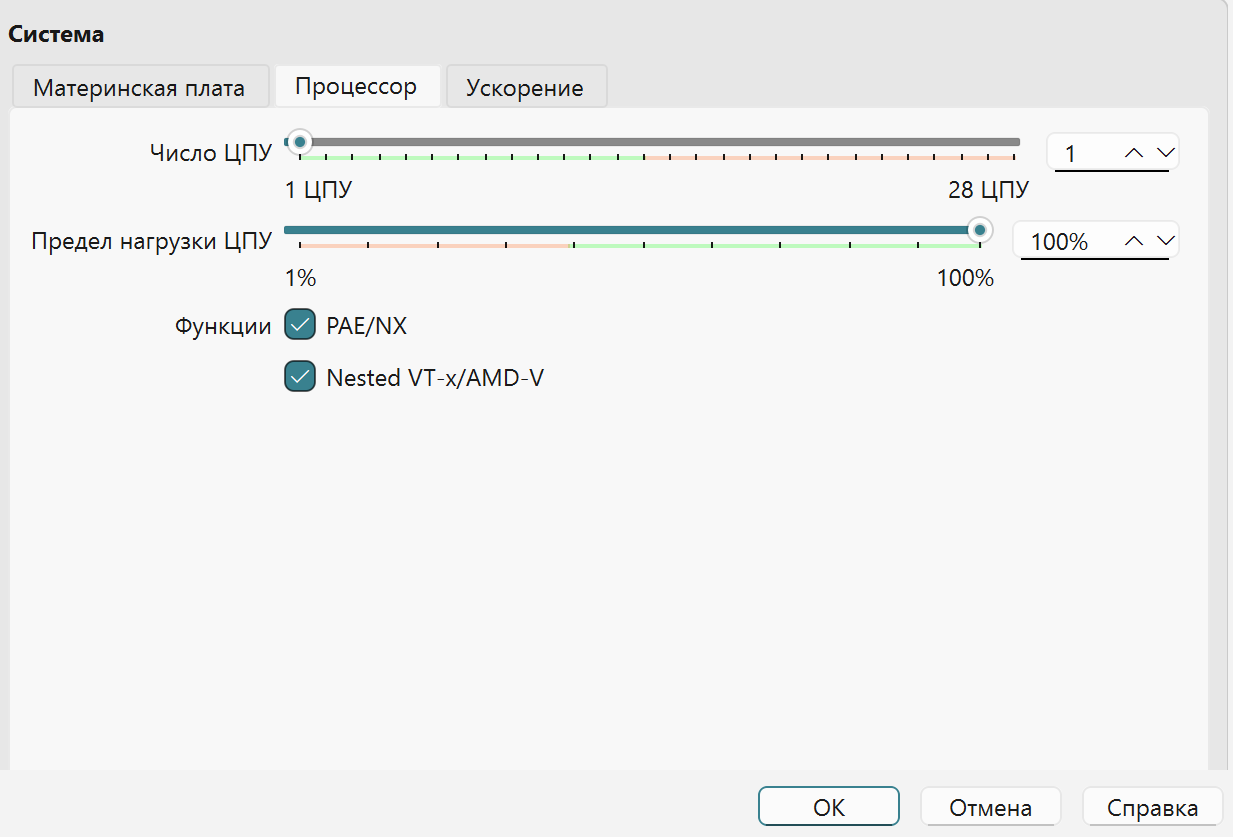
\includegraphics[width=0.7\linewidth,height=\textheight,keepaspectratio]{image/8.png}

}

\caption{\label{fig-008}Настройка виртуально машины, вложенная
виртуализация}

\end{figure}%

Настроим сетевой адаптер. Для этого в VirtualBox выберем импортированную
виртуальную машину и перейдим к опции «Сеть» и во вкладке «Адаптер 1»
тип подключения должен быть установлен как «Виртуальный адаптер»
(рис.~\ref{fig-009}).

\begin{figure}

\centering{

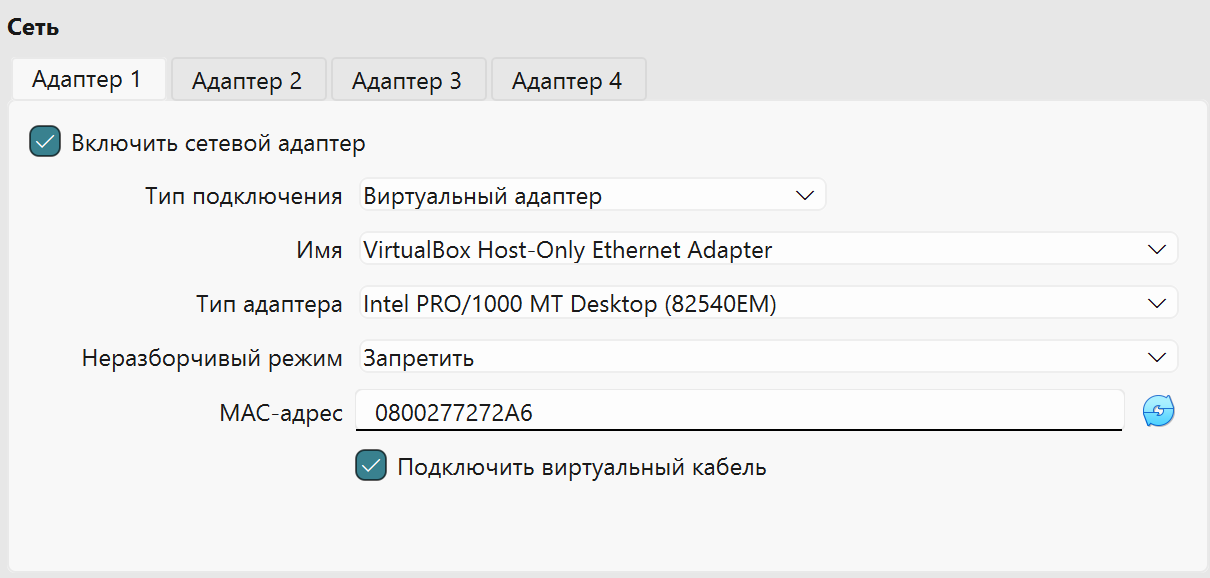
\includegraphics[width=0.7\linewidth,height=\textheight,keepaspectratio]{image/9.png}

}

\caption{\label{fig-009}Настройка виртуально машины, сетевой адаптер}

\end{figure}%

\section{Запуск экземпляра GNS3 в
VirtualBox}\label{ux437ux430ux43fux443ux441ux43a-ux44dux43aux437ux435ux43cux43fux43bux44fux440ux430-gns3-ux432-virtualbox}

Запустим GNS3 VM в VirtualBox (рис.~\ref{fig-010}).

\begin{figure}

\centering{

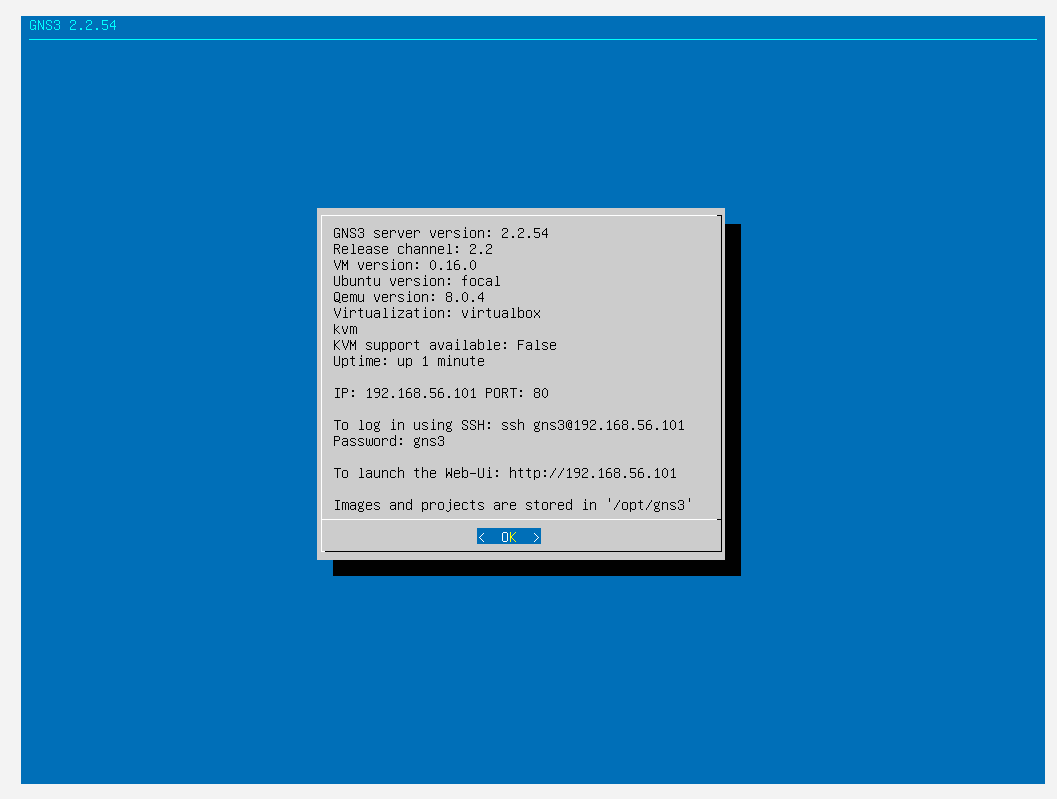
\includegraphics[width=0.7\linewidth,height=\textheight,keepaspectratio]{image/10.png}

}

\caption{\label{fig-010}Запуск GNS3 VM в VirtualBox}

\end{figure}%

Затем в основной операционной системе запустим приложение gns3. При
первом запуске приложения gns3 запускается мастер настройки
(рис.~\ref{fig-011}).

\begin{figure}

\centering{

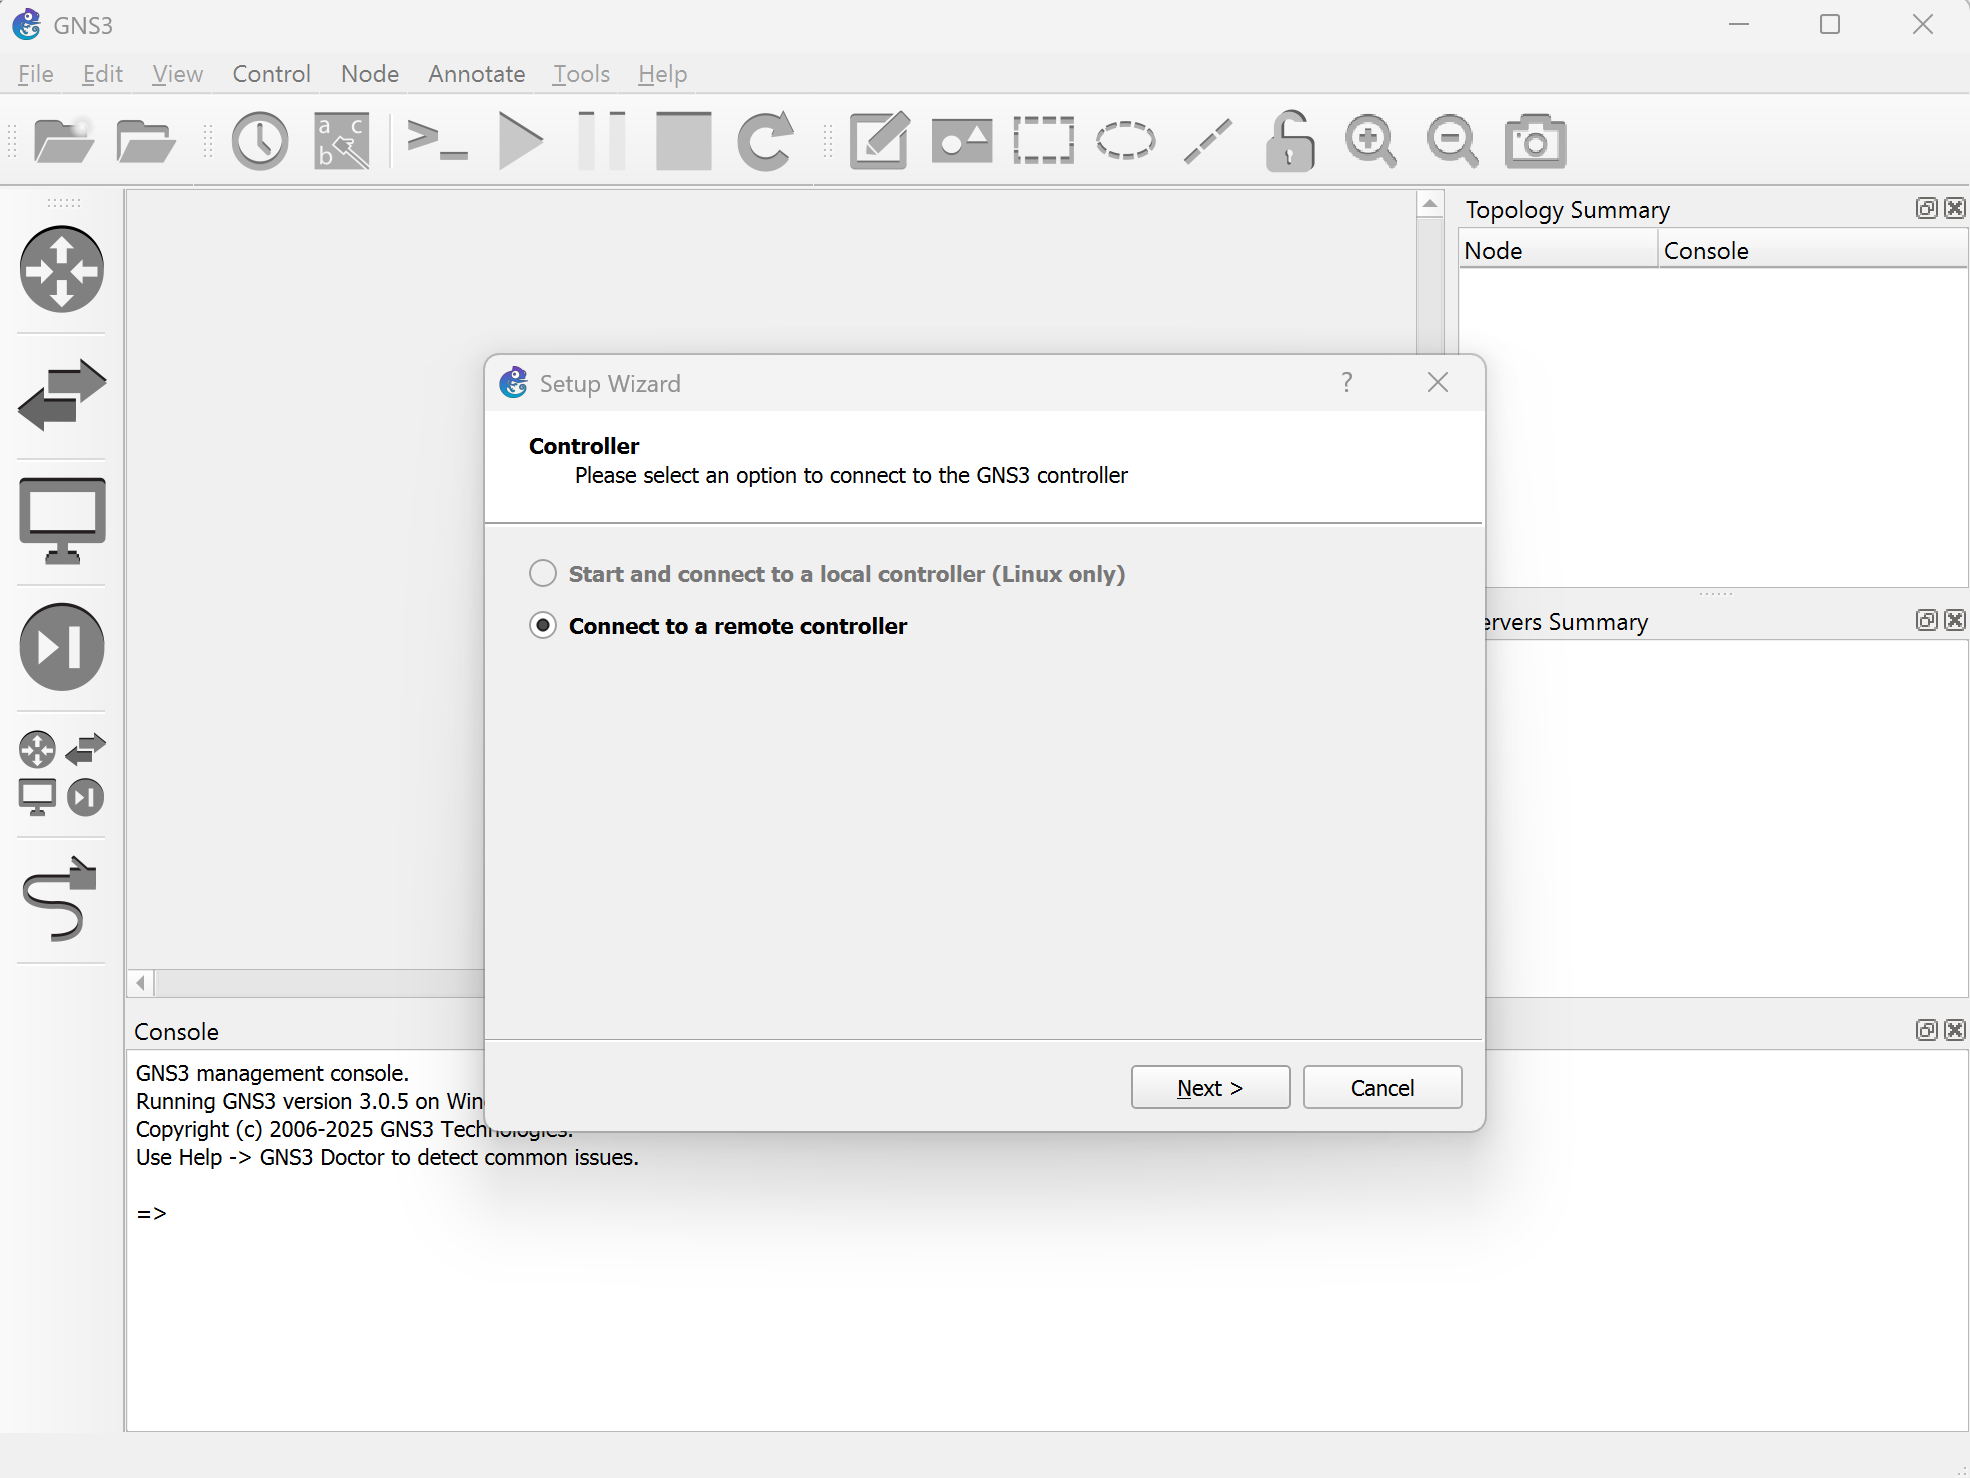
\includegraphics[width=0.7\linewidth,height=\textheight,keepaspectratio]{image/11.png}

}

\caption{\label{fig-011}Запуск GNS3}

\end{figure}%

В следующем окне указываются настройки локального сервера. Путь к
серверу и порт пишем как в нашей виртуальной машине, затем нажмаем Next
(рис.~\ref{fig-012}).

\begin{figure}

\centering{

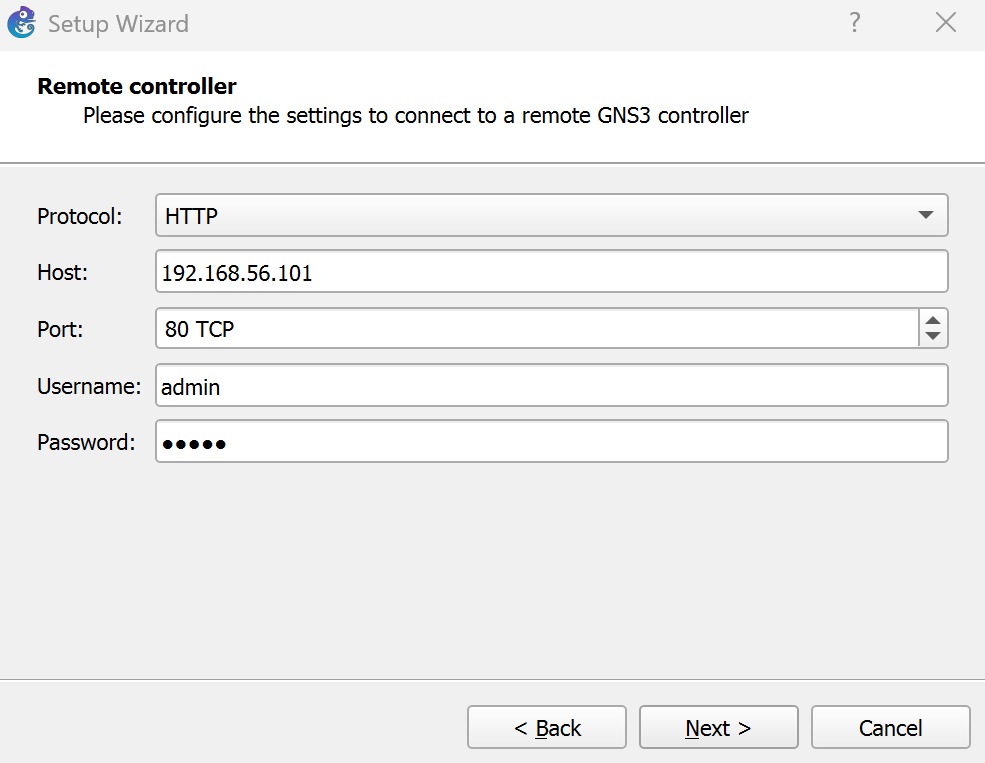
\includegraphics[width=0.7\linewidth,height=\textheight,keepaspectratio]{image/12.png}

}

\caption{\label{fig-012}Настройки локального сервера}

\end{figure}%

После успешного подсоединения должно появиться окно с итоговыми
настройками, на котором следует нажать Finish (рис.~\ref{fig-013}).

\begin{figure}

\centering{

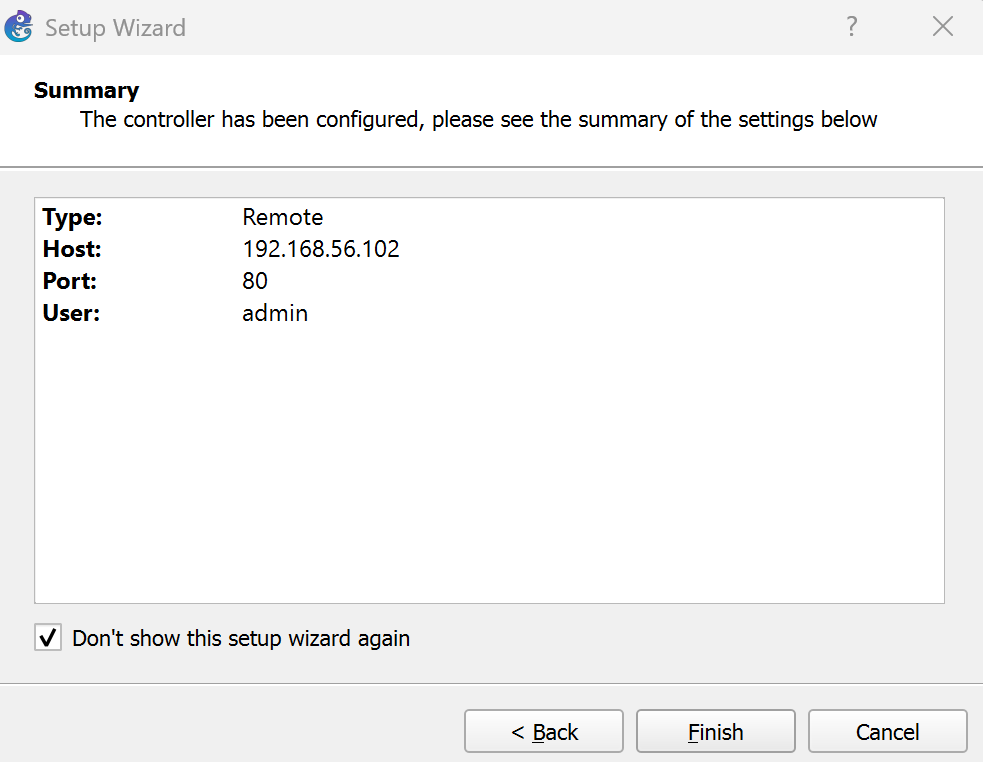
\includegraphics[width=0.7\linewidth,height=\textheight,keepaspectratio]{image/13.png}

}

\caption{\label{fig-013}Итоговые настройки}

\end{figure}%

\section{Выключение
GNS3}\label{ux432ux44bux43aux43bux44eux447ux435ux43dux438ux435-gns3}

Выключать GNS3 следует через меню File Quit . При этом виртуальная
машина GNS VM должна выключится сама, но к сожалению, как я узнала в
интернете, в современной версии программы это не всегда работает
(рис.~\ref{fig-014}).

\begin{figure}

\centering{

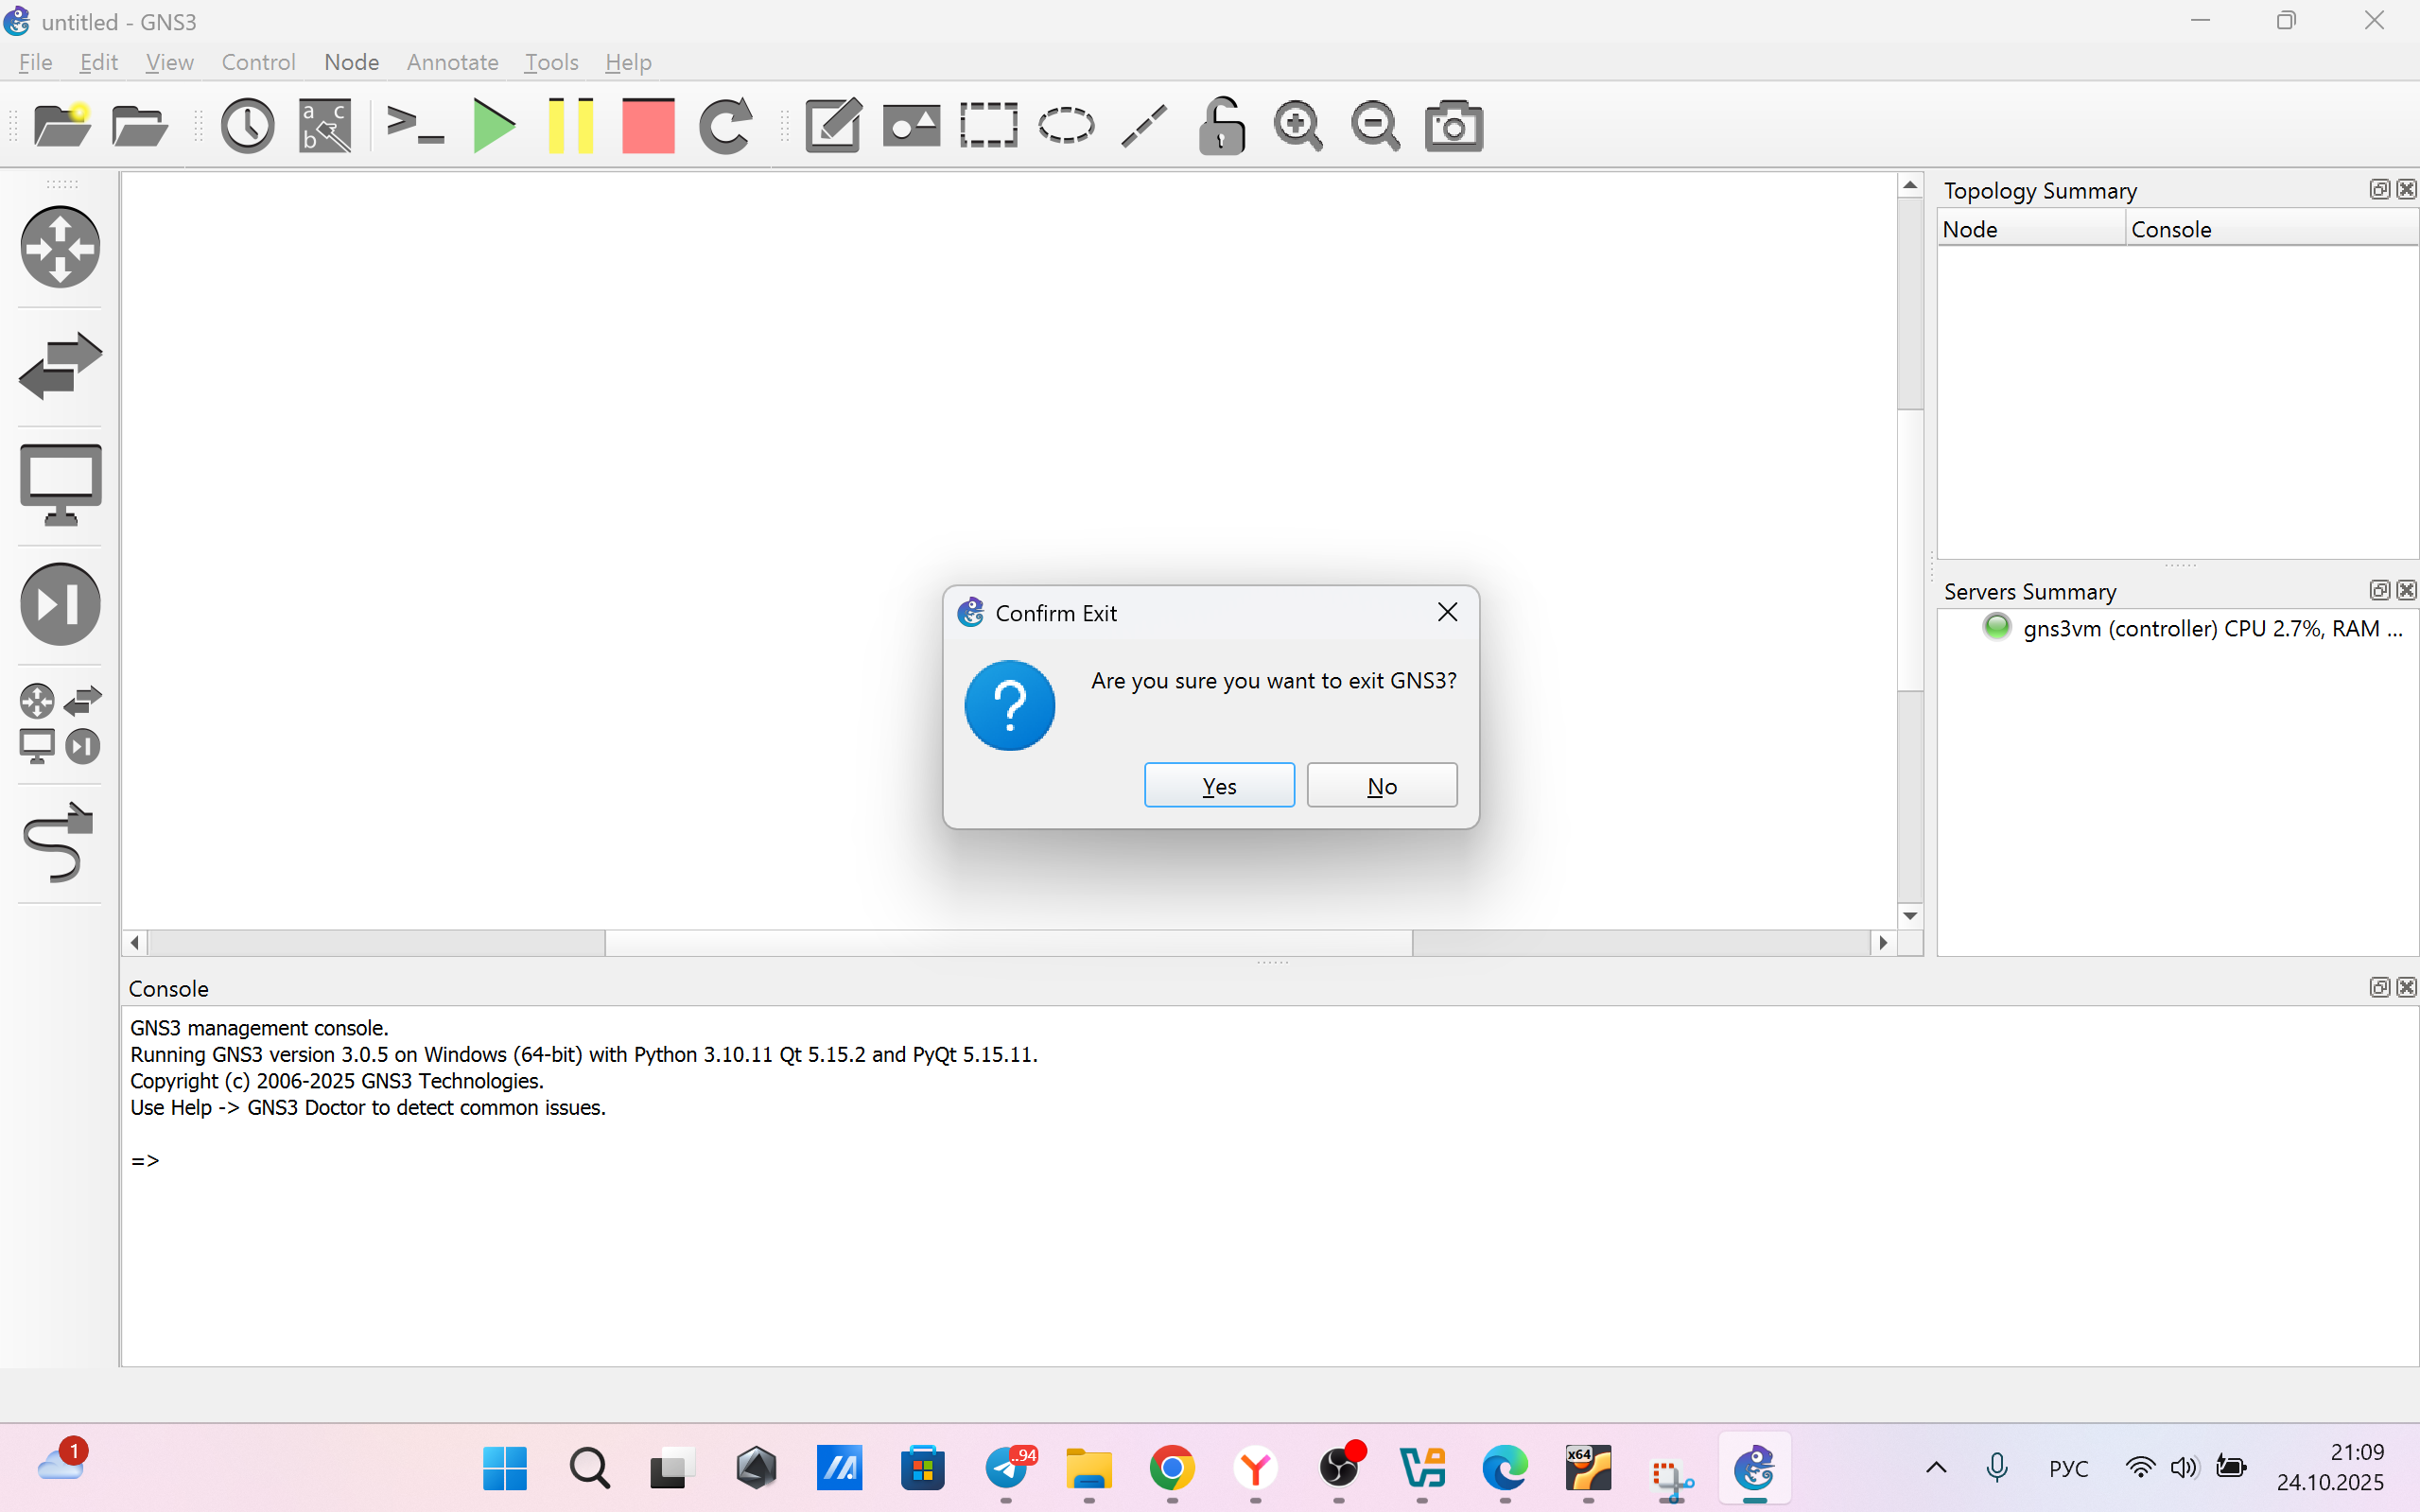
\includegraphics[width=0.7\linewidth,height=\textheight,keepaspectratio]{image/14.png}

}

\caption{\label{fig-014}Попытка выключения}

\end{figure}%

\section{Добавление образа маршрутизатора
FRR}\label{ux434ux43eux431ux430ux432ux43bux435ux43dux438ux435-ux43eux431ux440ux430ux437ux430-ux43cux430ux440ux448ux440ux443ux442ux438ux437ux430ux442ux43eux440ux430-frr}

Предположим, что требуется добавить образ маршрутизатора (FRRouting). В
рабочем пространстве GNS3 на левой боковой панели выберем просмотр
маршрутизаторов (Browse Routers), затем нажмём на + New template. В
открывшемся окне укажем рекомендуемое верхнее значение, а именно,
устанавливать образ с GNS3-сервера (рис.~\ref{fig-015})

\begin{figure}

\centering{

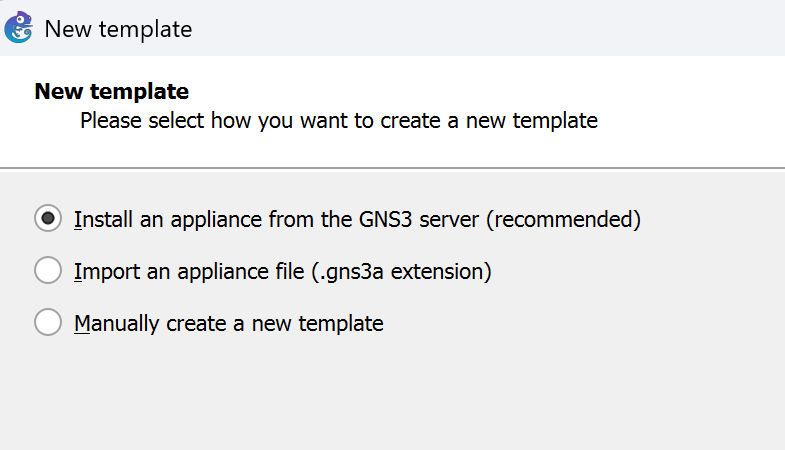
\includegraphics[width=0.7\linewidth,height=\textheight,keepaspectratio]{image/15.png}

}

\caption{\label{fig-015}Добавление образа маршрутизатора FRR}

\end{figure}%

В следующем окне выбираем Routers и образ FRR (FRRouting)
(рис.~\ref{fig-016}).

\begin{figure}

\centering{

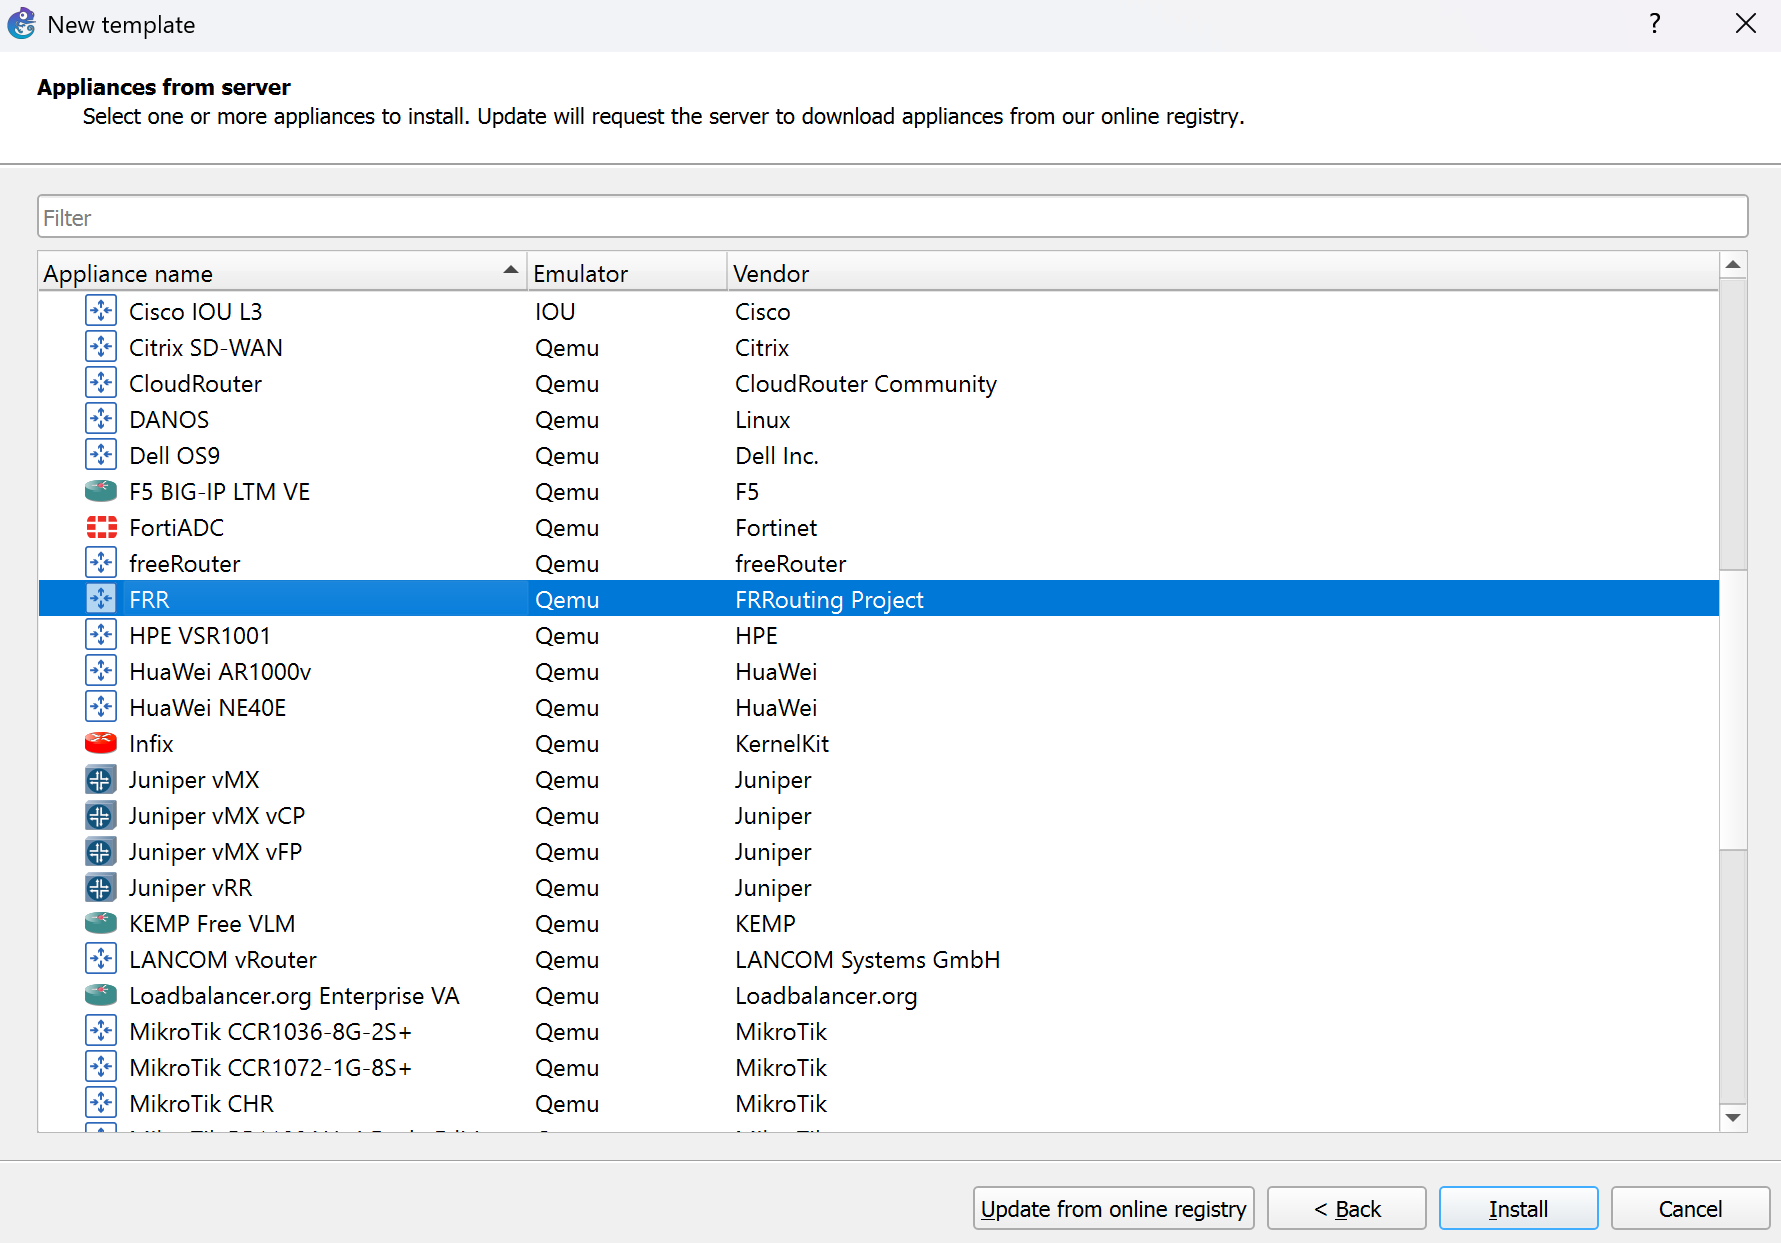
\includegraphics[width=0.7\linewidth,height=\textheight,keepaspectratio]{image/16.png}

}

\caption{\label{fig-016}Выбор образа FRR}

\end{figure}%

В следующем окне предлагается перечень файлов для скачивания и
последующей установки. Скачиваю версию 8.2.2 и импортирую образ
(рис.~\ref{fig-017}).

\begin{figure}

\centering{

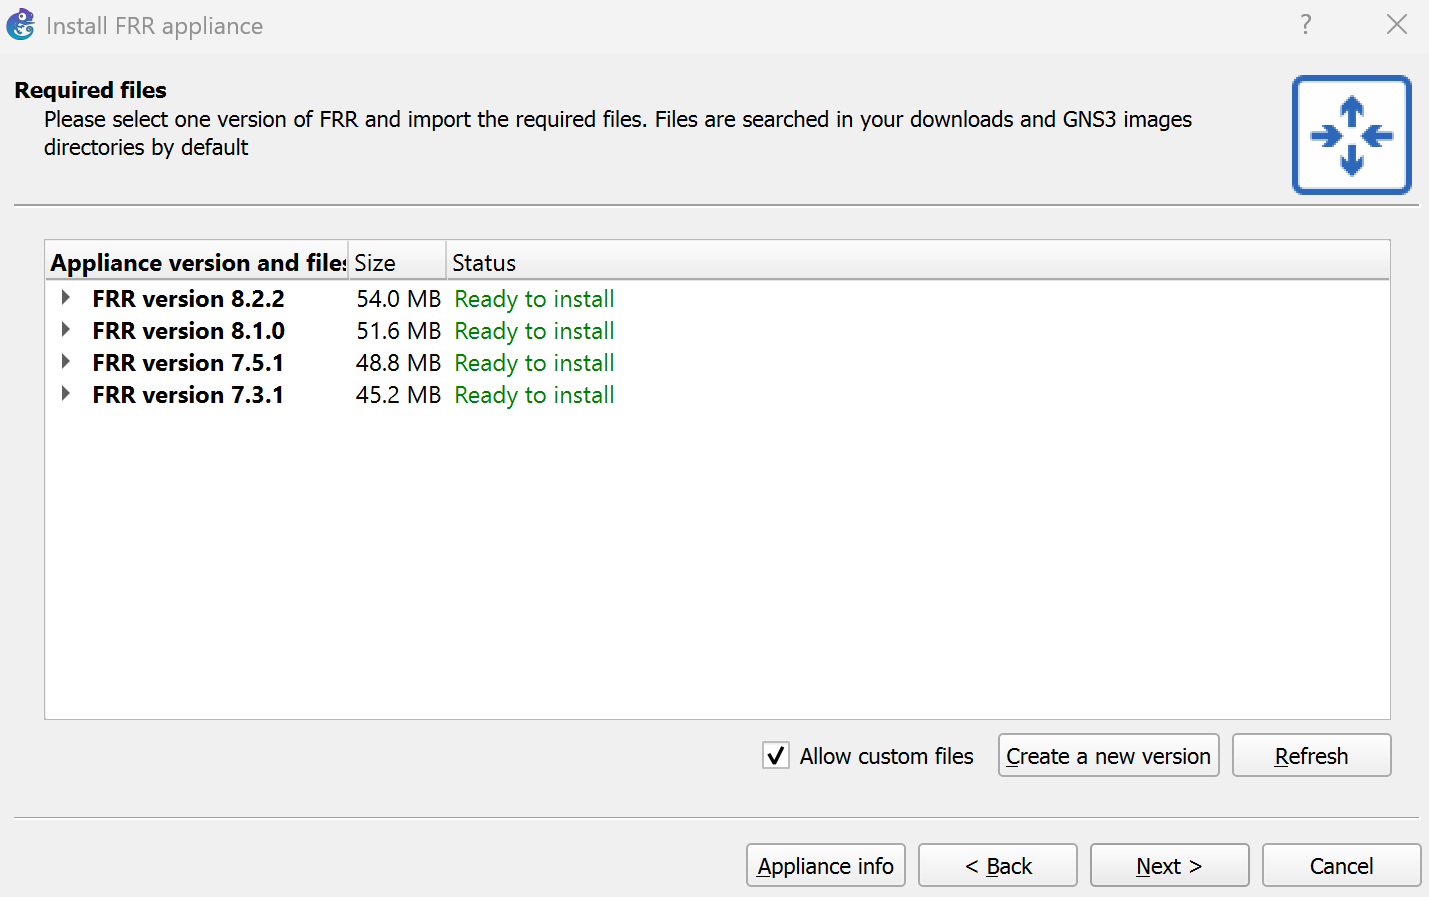
\includegraphics[width=0.7\linewidth,height=\textheight,keepaspectratio]{image/17.png}

}

\caption{\label{fig-017}Скачивание необходимых файлов}

\end{figure}%

На заключительном окне указывается краткая информация об устройстве,
просмотрим её и нажмём Finish (рис.~\ref{fig-018}).

\begin{figure}

\centering{

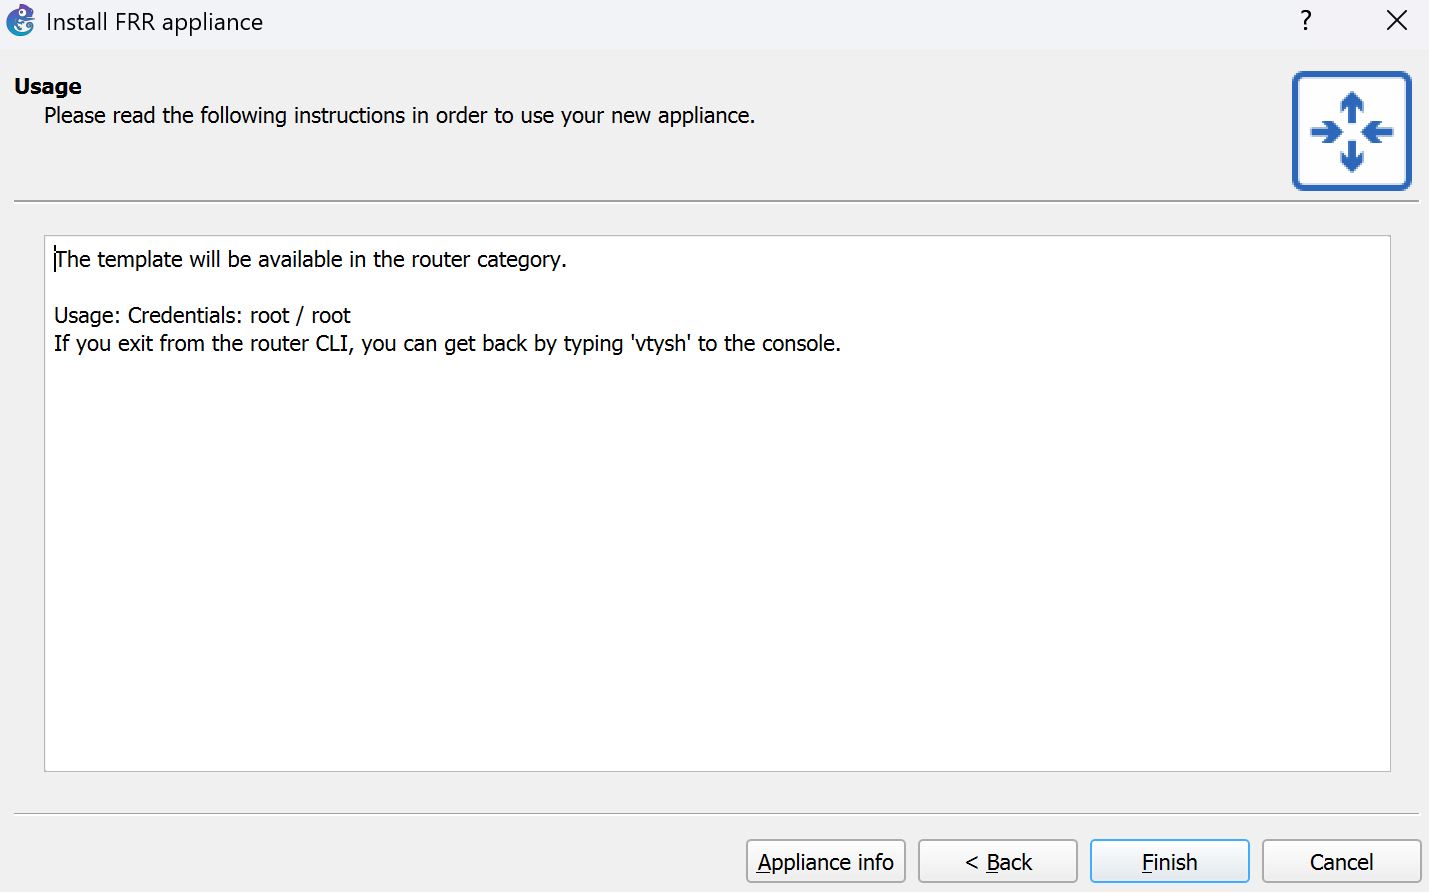
\includegraphics[width=0.7\linewidth,height=\textheight,keepaspectratio]{image/18.png}

}

\caption{\label{fig-018}Краткая информация об устройстве}

\end{figure}%

В рабочем пространстве на левой панели в списке маршрутизаторов появится
образ устройства FRR. (рис.~\ref{fig-019}).

\begin{figure}

\centering{

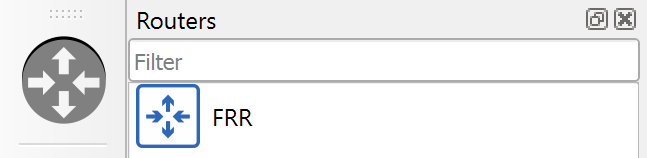
\includegraphics[width=0.7\linewidth,height=\textheight,keepaspectratio]{image/19.png}

}

\caption{\label{fig-019}Значок образа устройства FRR}

\end{figure}%

Далее необходимо настроить образ маршрутизатора. Правой кнопкой мыши
щёлкаем на образе устройства, в меню выбираем Configure template. В
открывшемся окне необходимо во вкладке «General settings» в поле «On
close» выбрать Send the shutdown signal (ACPI) (рис.~\ref{fig-020}).

\begin{figure}

\centering{

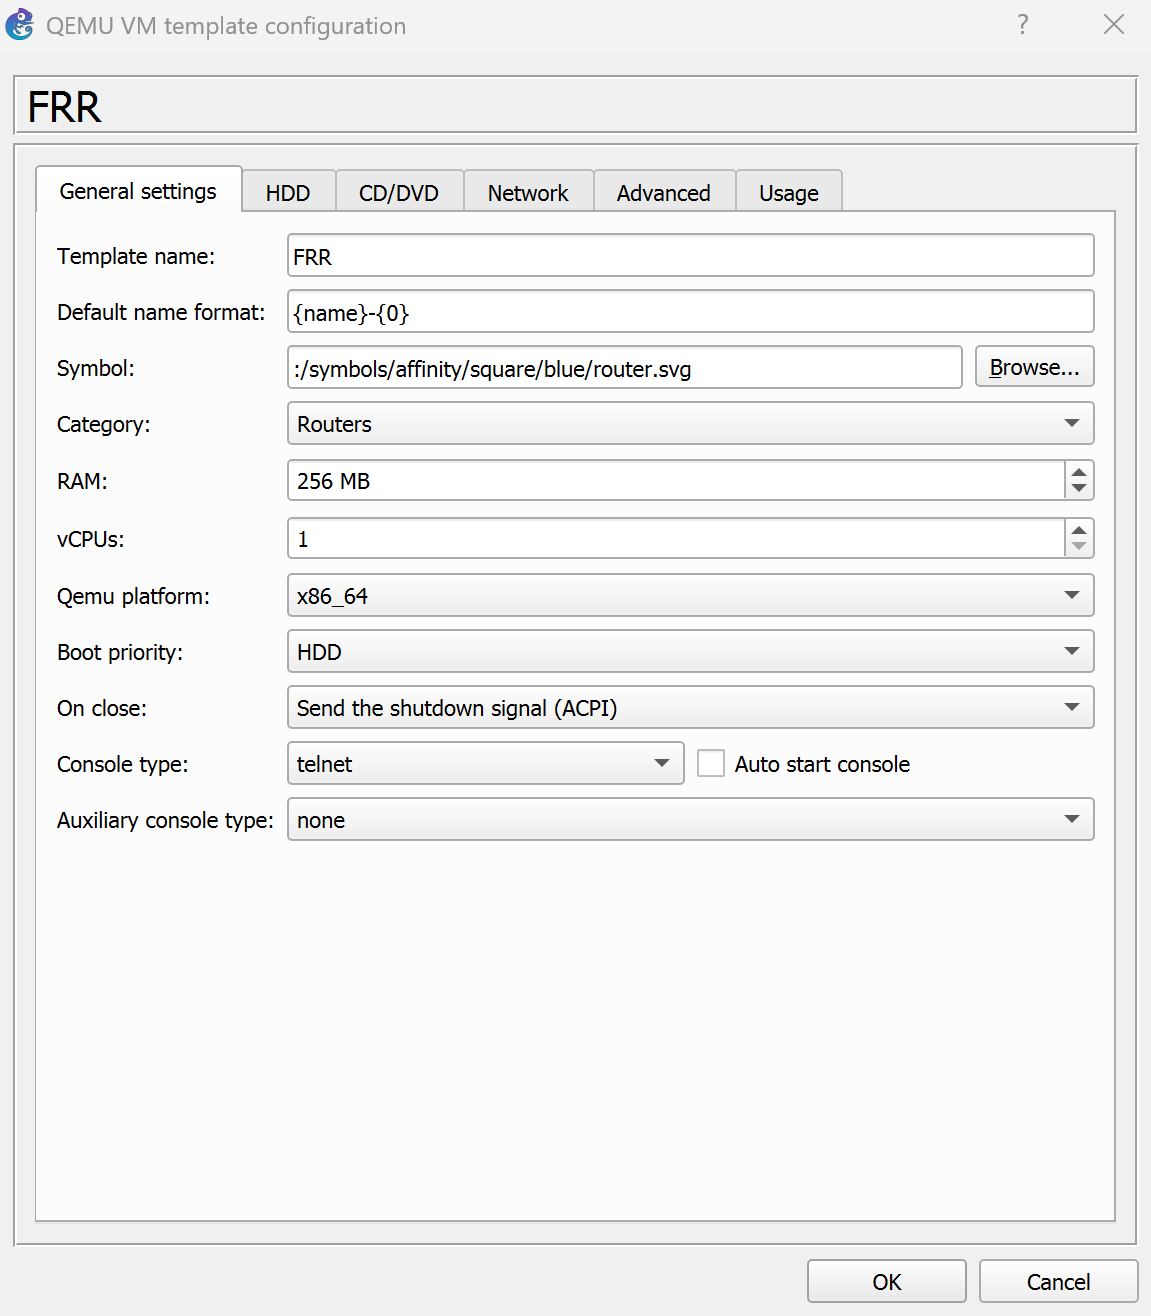
\includegraphics[width=0.7\linewidth,height=\textheight,keepaspectratio]{image/20.png}

}

\caption{\label{fig-020}Настройка образа маршрутизатора, General
settings}

\end{figure}%

Во вкладке «HDD» необходимо поставить галочку «Automatically create a
config disk on HDD» (рис.~\ref{fig-021}).

\begin{figure}

\centering{

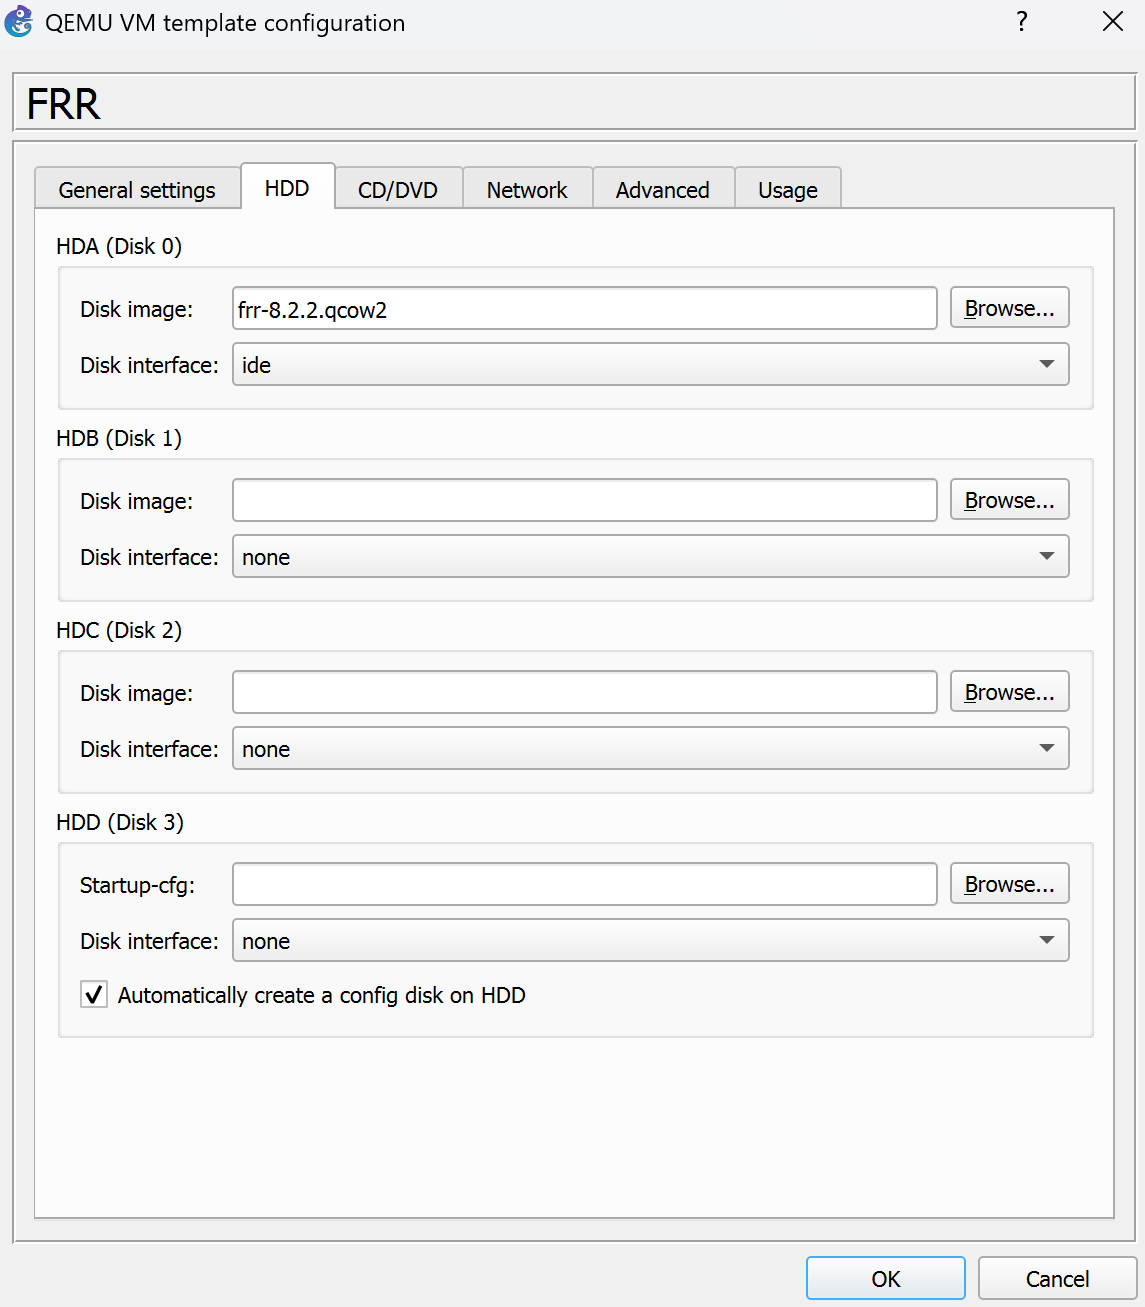
\includegraphics[width=0.7\linewidth,height=\textheight,keepaspectratio]{image/21.png}

}

\caption{\label{fig-021}Настройка образа маршрутизатора, HDD}

\end{figure}%

\section{Добавление образа маршрутизатора
VyOS}\label{ux434ux43eux431ux430ux432ux43bux435ux43dux438ux435-ux43eux431ux440ux430ux437ux430-ux43cux430ux440ux448ux440ux443ux442ux438ux437ux430ux442ux43eux440ux430-vyos}

Требуется добавить образ маршрутизатора VyOS. В рабочем пространстве
GNS3 на левой боковой панели выберем просмотр маршрутизаторов (Browse
Routers), затем нажмём на + New template. В открывшемся окне укажем
рекомендуемое верхнее значение, а именно, устанавливать образ с
GNS3-сервера (рис.~\ref{fig-022}).

\begin{figure}

\centering{

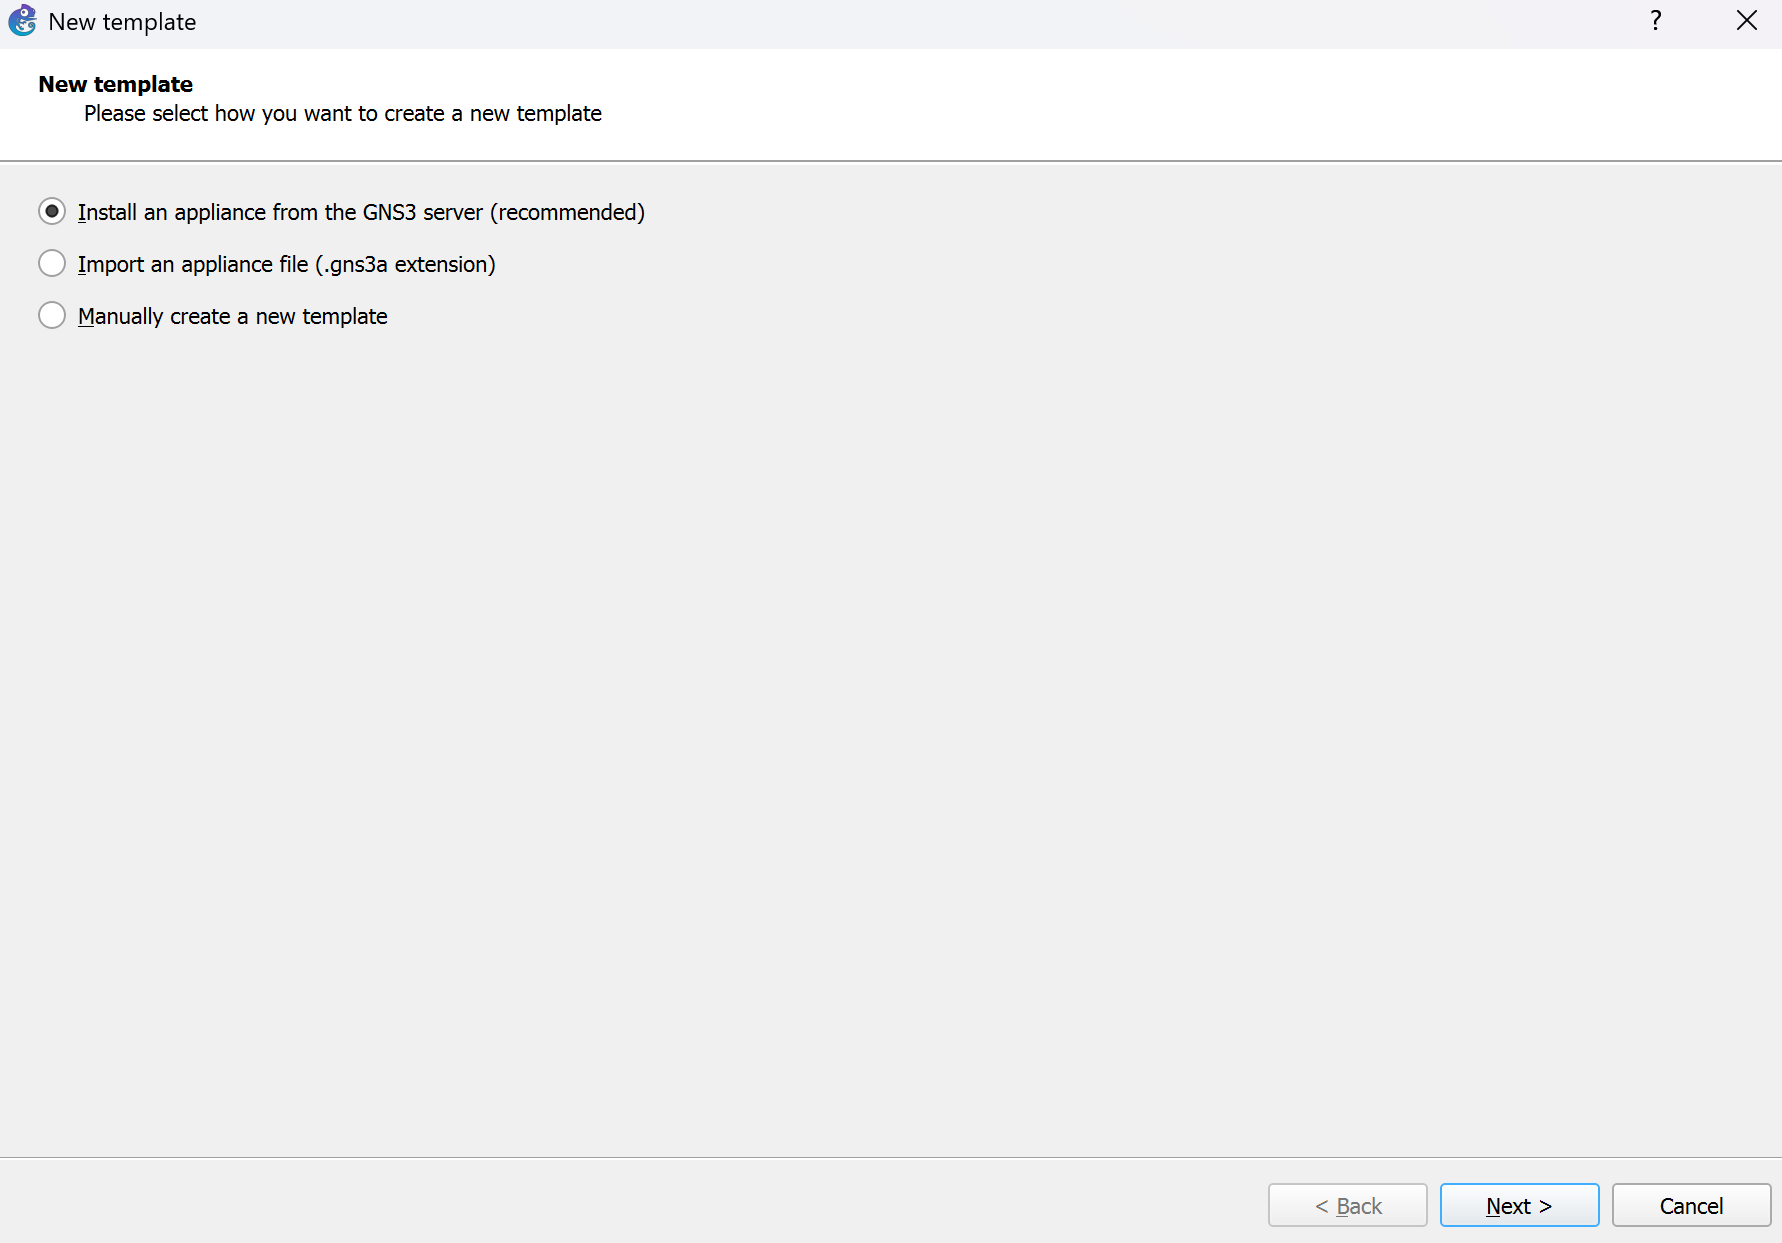
\includegraphics[width=0.7\linewidth,height=\textheight,keepaspectratio]{image/22.png}

}

\caption{\label{fig-022}Добавление образа маршрутизатора VyOS}

\end{figure}%

В следующем окне выбираем Routers и образ VyOS (рис.~\ref{fig-023}).

\begin{figure}

\centering{

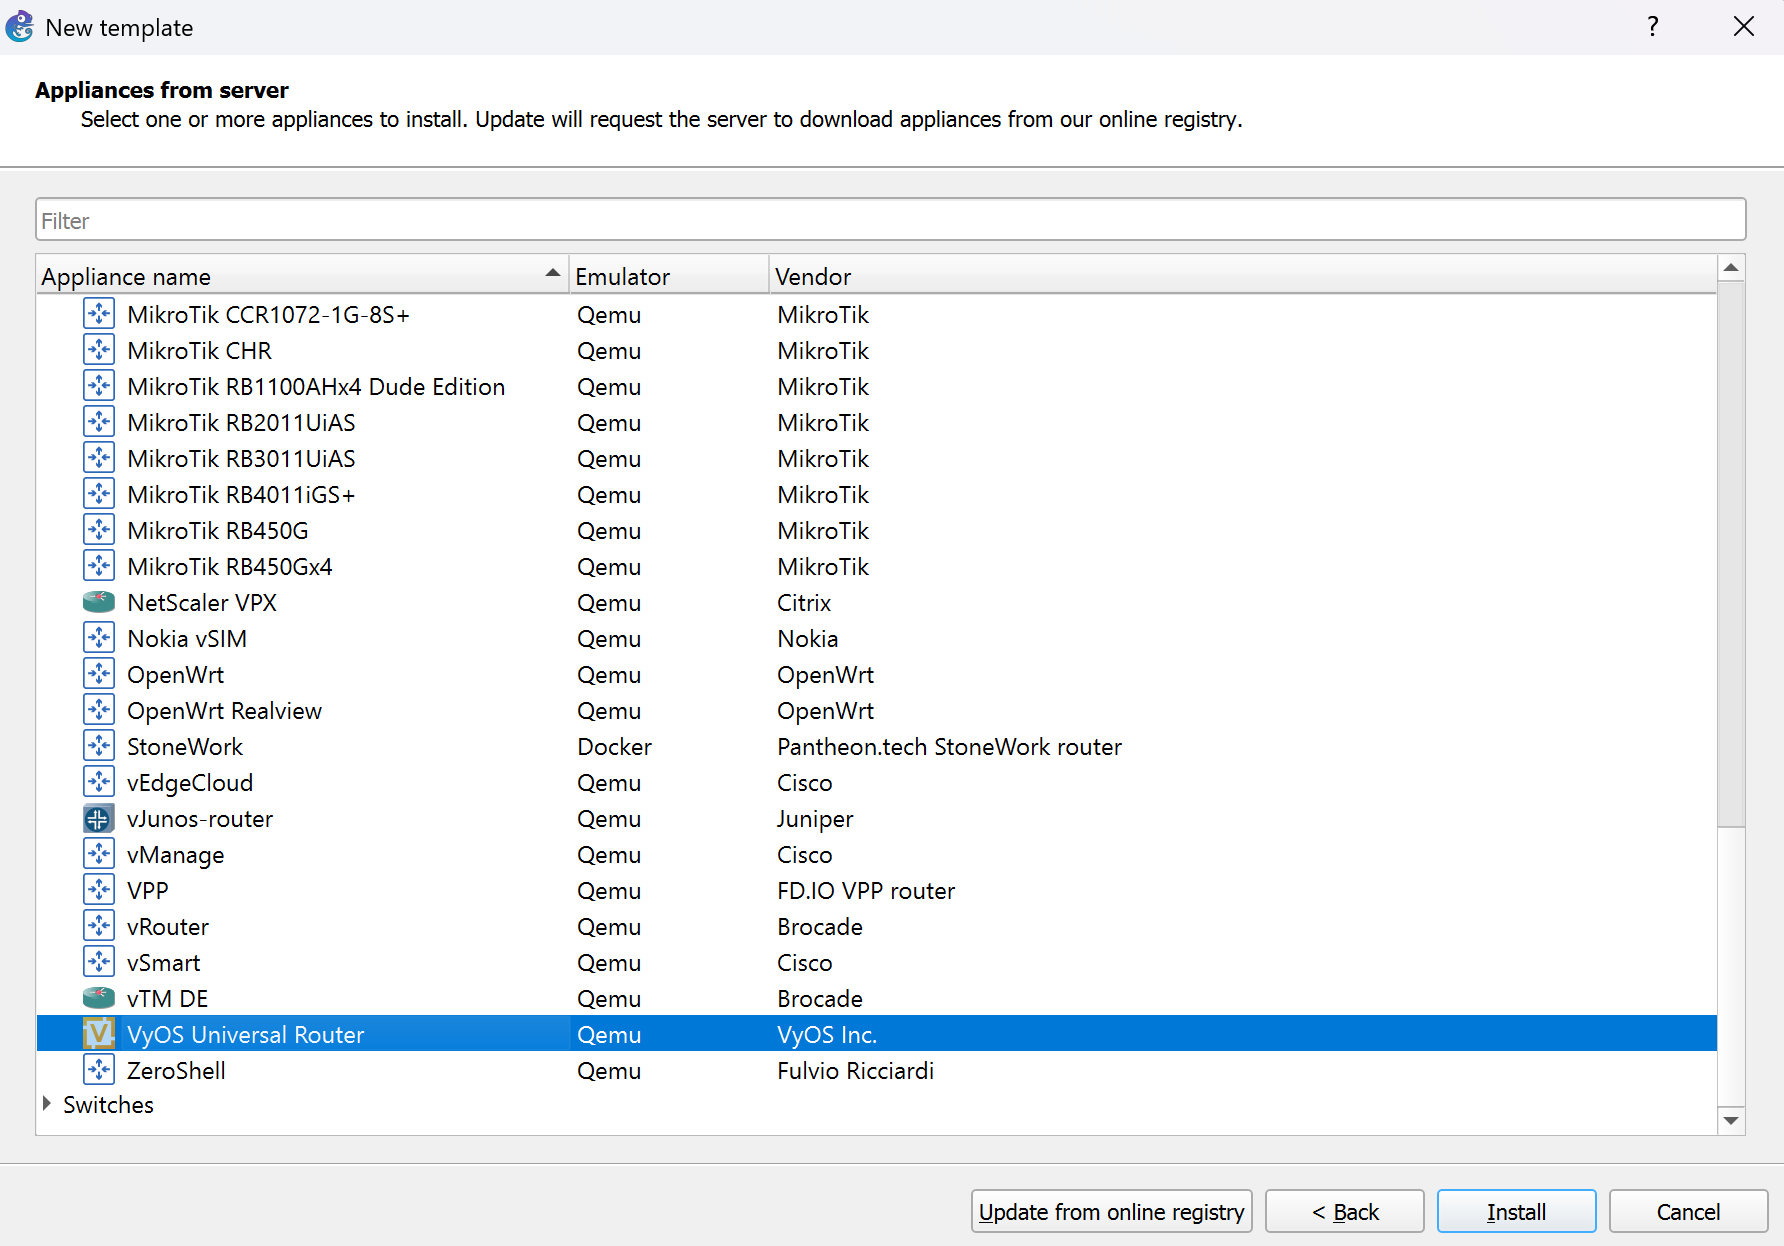
\includegraphics[width=0.7\linewidth,height=\textheight,keepaspectratio]{image/23.png}

}

\caption{\label{fig-023}Выбор образа VyOS}

\end{figure}%

В следующем окне предлагается перечень файлов для скачивания и
последующей установки. Скачиваю версию 1.3.3 которую сделала сама и
скачала с бесплатного сервиса и импортирую образ (рис.~\ref{fig-024}).

\begin{figure}

\centering{

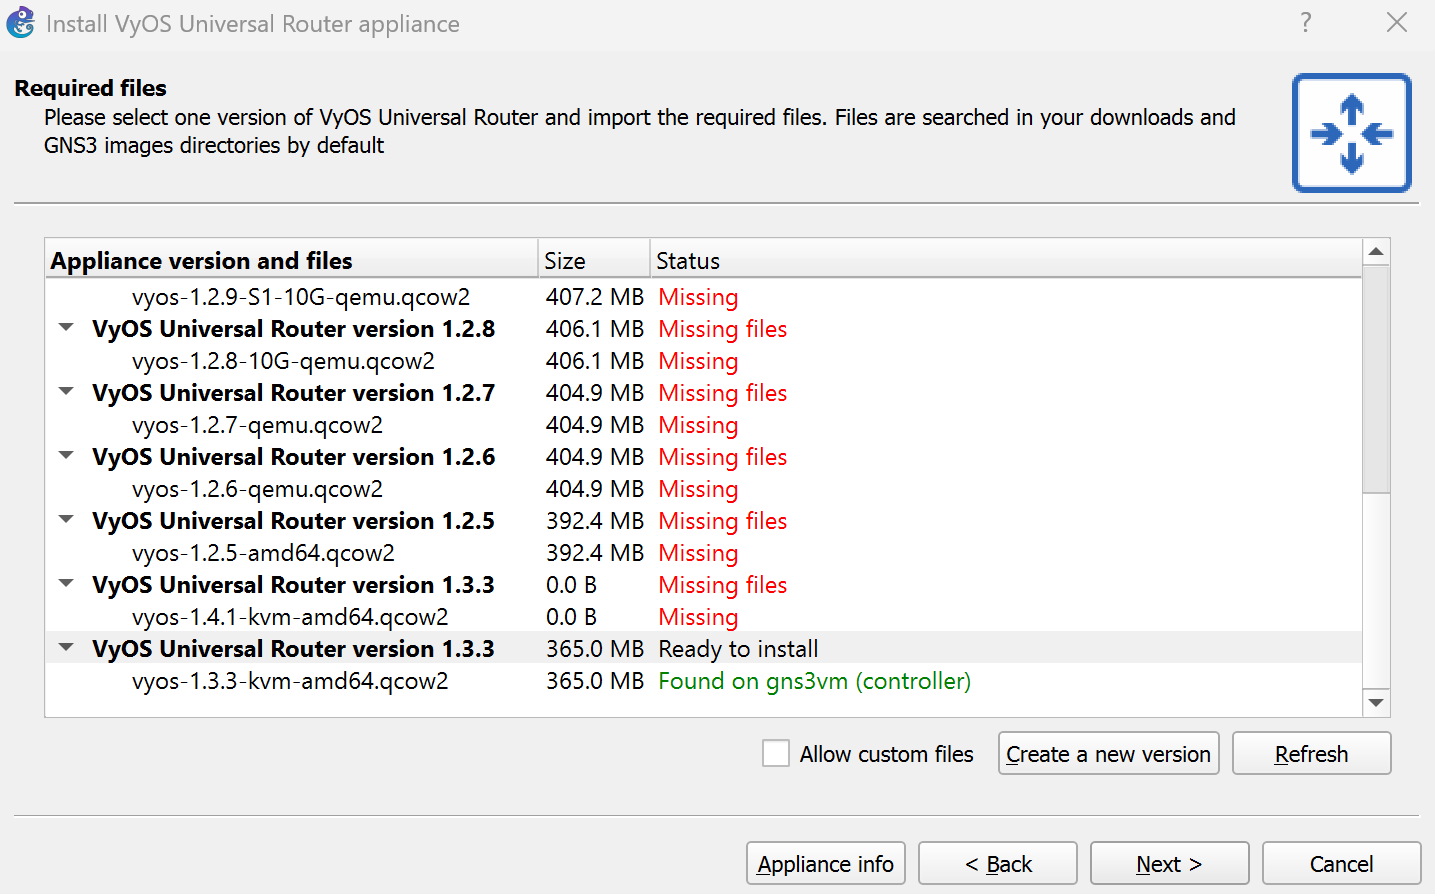
\includegraphics[width=0.7\linewidth,height=\textheight,keepaspectratio]{image/24.png}

}

\caption{\label{fig-024}Скачивание необходимых файлов}

\end{figure}%

На заключительном окне указывается краткая информация об устройстве,
просмотрим её и нажмём Finish (рис.~\ref{fig-025}).

\begin{figure}

\centering{

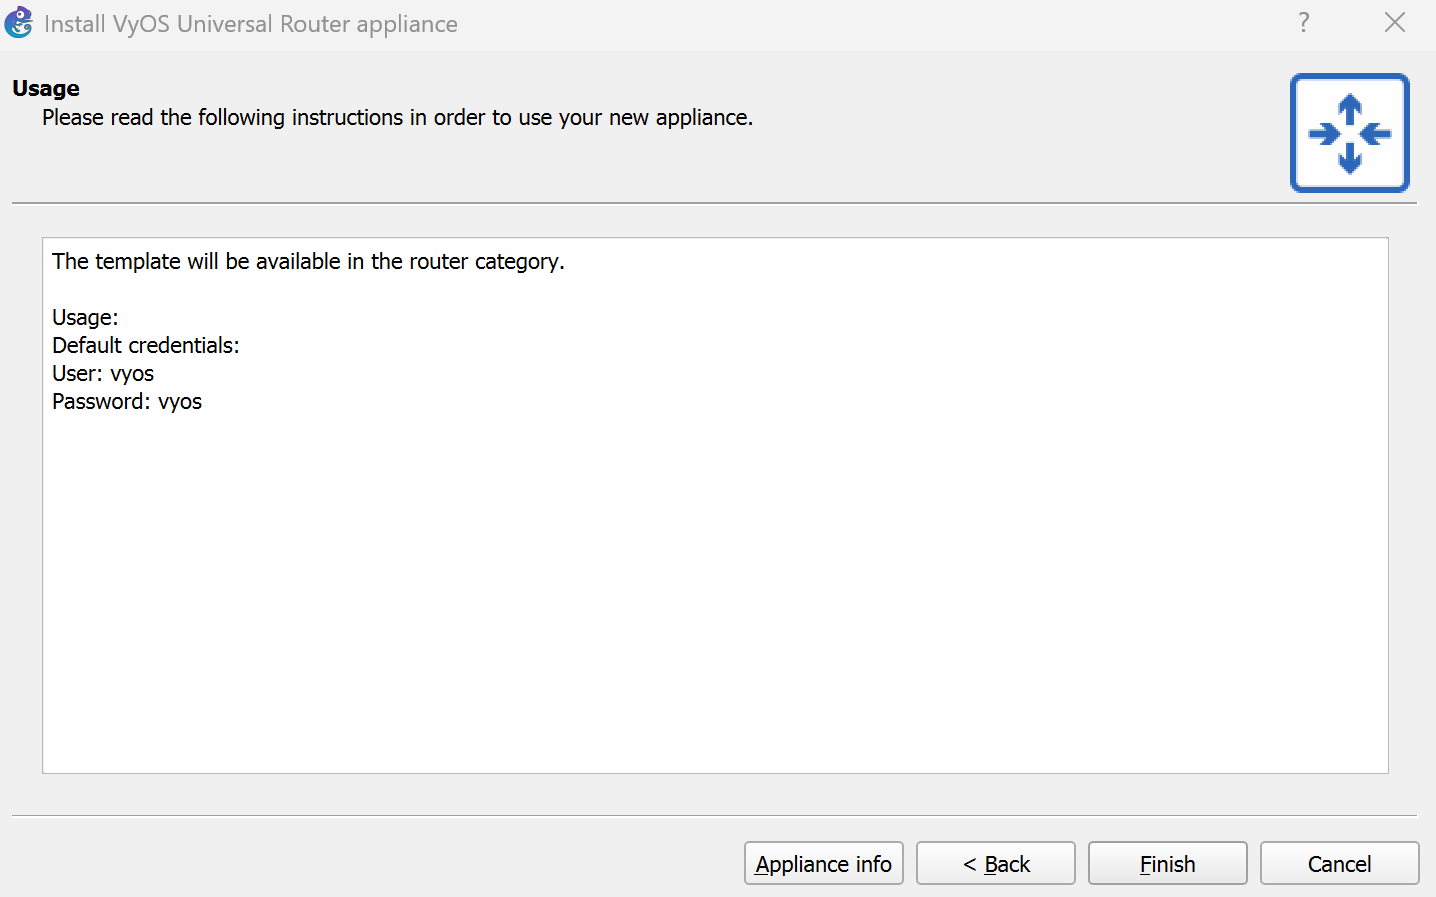
\includegraphics[width=0.7\linewidth,height=\textheight,keepaspectratio]{image/25.png}

}

\caption{\label{fig-025}Краткая информация об устройстве}

\end{figure}%

В рабочем пространстве на левой панели в списке маршрутизаторов появится
образ устройства VyOS. (рис.~\ref{fig-026}).

\begin{figure}

\centering{

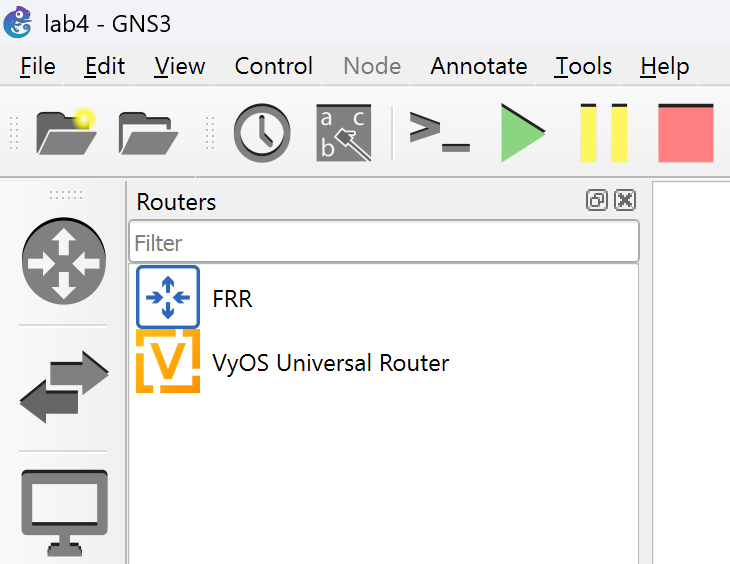
\includegraphics[width=0.7\linewidth,height=\textheight,keepaspectratio]{image/26.png}

}

\caption{\label{fig-026}Значок образа устройства VyOS}

\end{figure}%

Далее необходимо настроить образ маршрутизатора. Правой кнопкой мыши
щёлкаем на образе устройства, в меню выбираем Configure template. В
открывшемся окне необходимо во вкладке «General settings» в поле «On
close» выбрать Send the shutdown signal (ACPI) (рис.~\ref{fig-027}).

\begin{figure}

\centering{

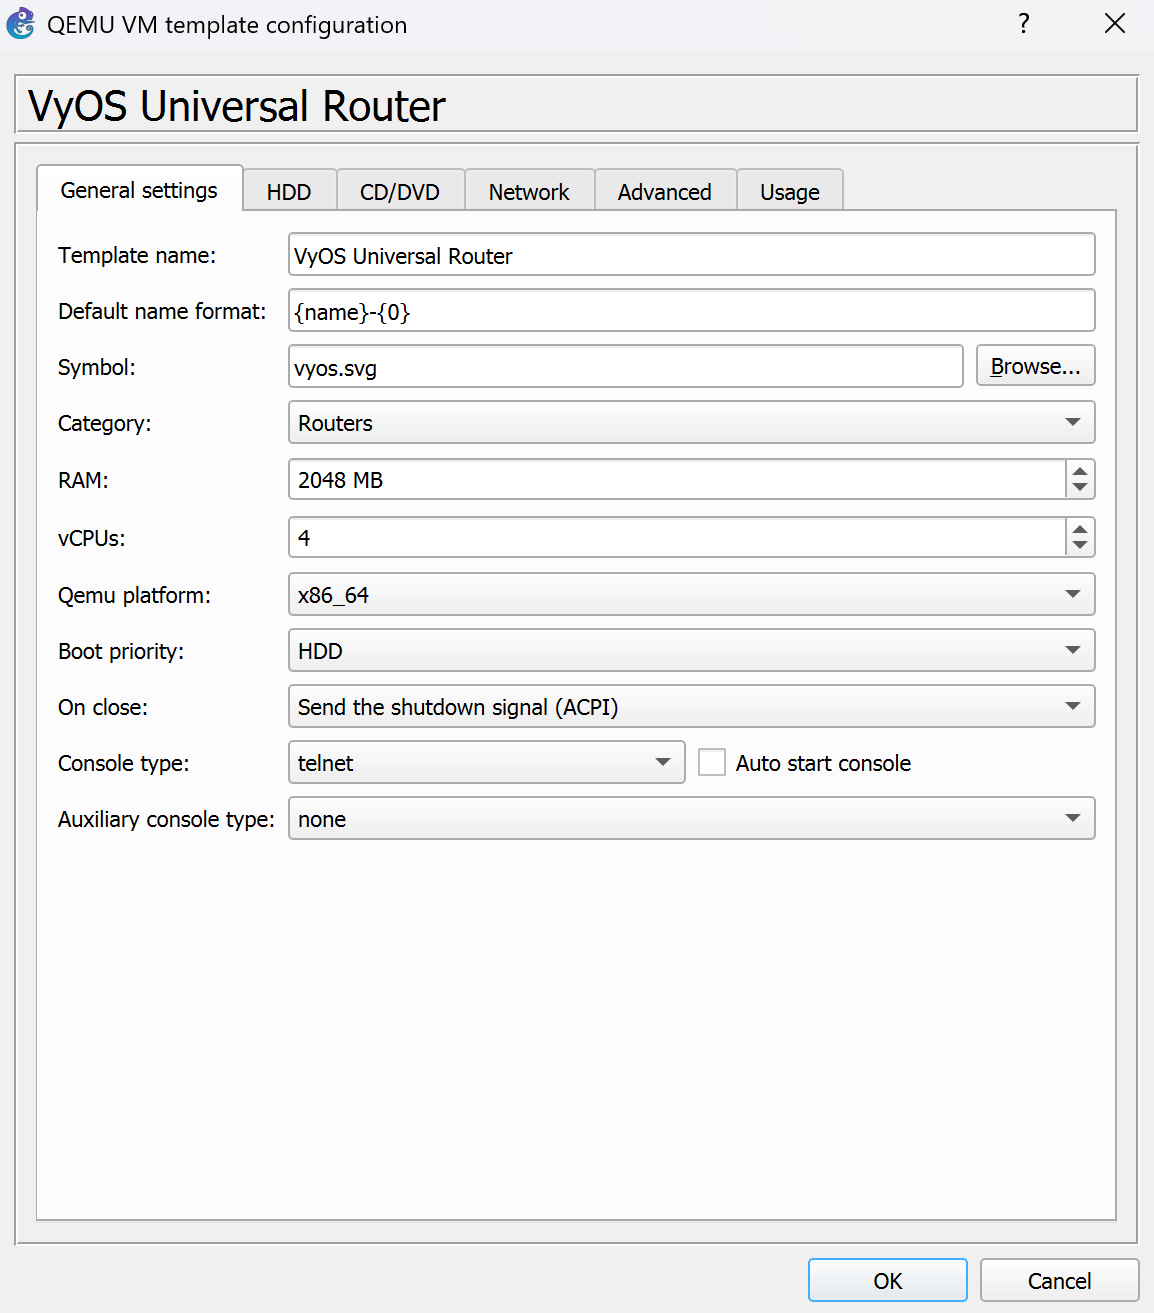
\includegraphics[width=0.7\linewidth,height=\textheight,keepaspectratio]{image/27.png}

}

\caption{\label{fig-027}Настройка образа маршрутизатора, General
settings}

\end{figure}%

Во вкладке «HDD» необходимо поставить галочку «Automatically create a
config disk on HDD» (рис.~\ref{fig-028}).

\begin{figure}

\centering{

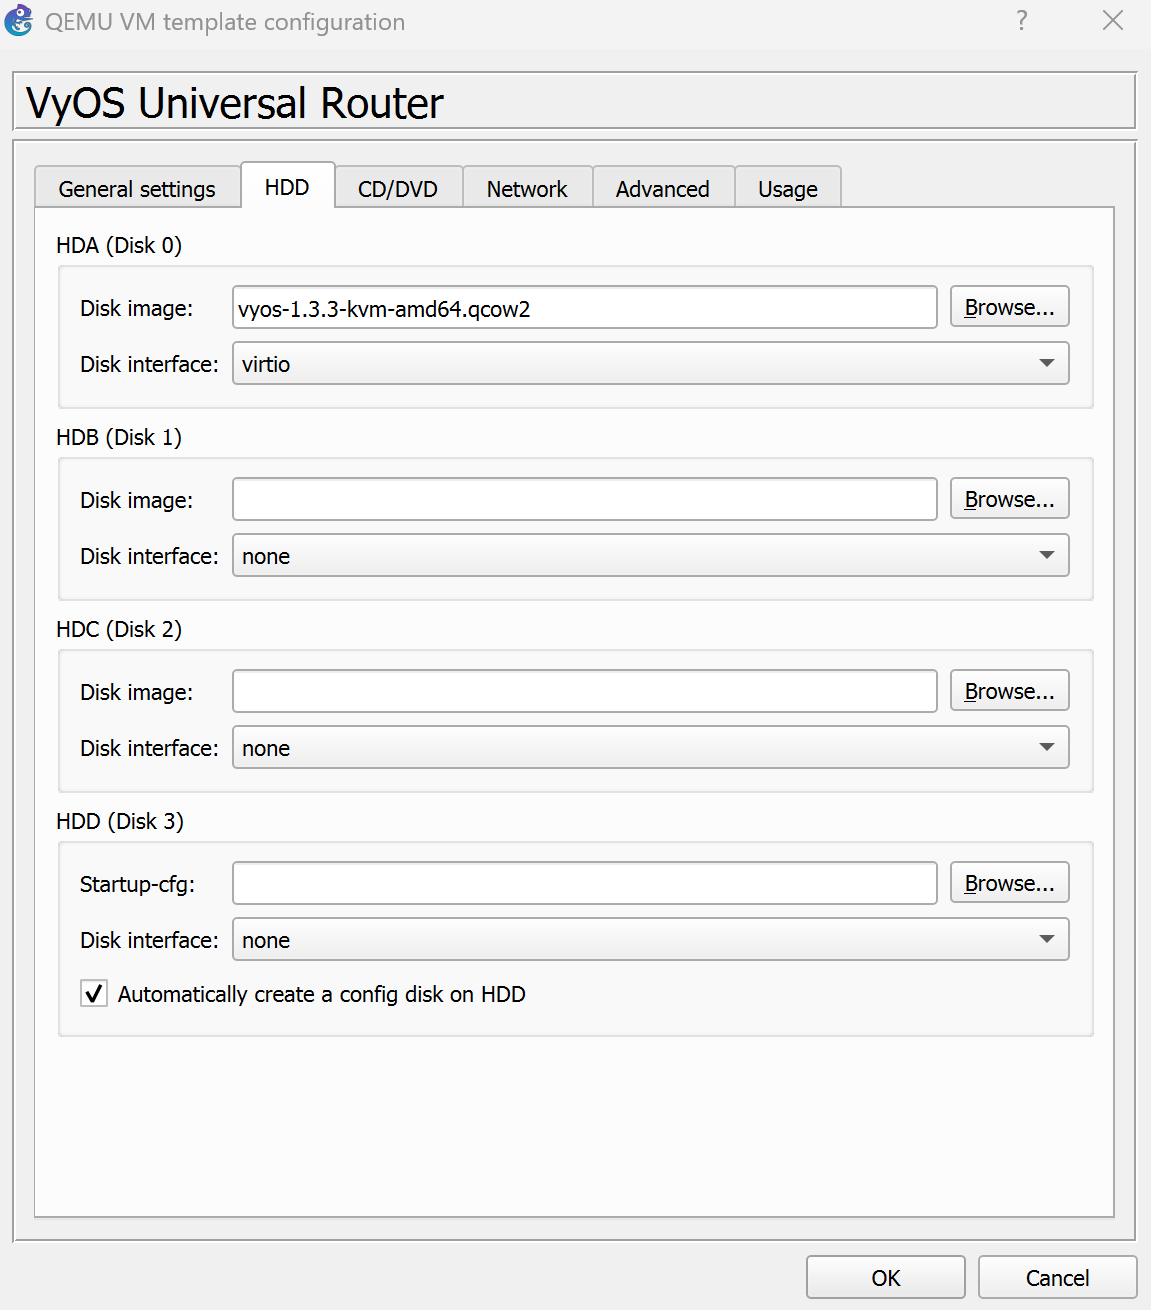
\includegraphics[width=0.7\linewidth,height=\textheight,keepaspectratio]{image/28.png}

}

\caption{\label{fig-028}Настройка образа маршрутизатора, HDD}

\end{figure}%

\chapter{Выводы}\label{ux432ux44bux432ux43eux434ux44b}

В ходе выполнения лабораторной работы были получены навыки установка и
настройка GNS3 и сопутствующего программного обеспечения.


\printbibliography



\end{document}
